\providecommand{\main}{..}
\documentclass[\main/main.tex]{subfiles}

\begin{document}
\graphicspath{{img/}{03_firmware/img/}}

\chapter{Ranging system architecture}
This section provides a detailed description of the ranging network operation and layered system architecture.

\section{Prerequisite}
Before getting into, we should cover some fundamental definitions. It will make it easier for further discussions. 

\subsection{Host and device}
The implemented UWB ranging system consists of one host and one device.
\begin{itemize}
    \item Host: the MCU which control the radio IC 
    \item Device: the radio IC transmitting and receiving over-the-air packet
\end{itemize}

\begin{figure}[H]
    \begin{center}
        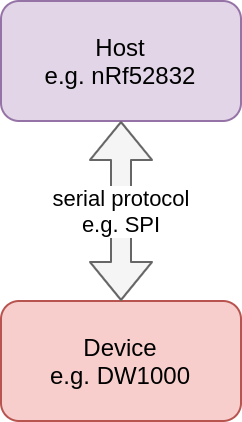
\includegraphics[width=0.2\textwidth]{host_device.png}
    \end{center}
    \caption{Host-device}
    \label{fig:host_device}
\end{figure}

\subsection{Timing system}
\label{subsec:timing_system_subsection}
Since there are two running systems: \textbf{host} and \textbf{device}, there are two timing systems. Unfortunately, these two timing systems do not have an agreement in the smallest unit of time. A host can use a $1\mu s$ -resolution timer due to the number of redundancy timers it has. A device, on the other hand, may not have as many timers and clock source as a host has, so the device timing system is limited. In the case of DW1000 radio IC, $1\mu s$ is approximately 512 counts of the fundamental 499.2 MHz UWB clock which is actually \textbf{$\sim 1.026\mu s$}. 

For precise timing, the implementation does not make any assumption about the equality of $1\mu s$ in host and device. Timestamp in the device must be converted to host reference for further processing, upon completion, the result must be converted back to the device reference before writing to that device. 
\subsection{RMarker}
Because of the limited transmission speed, the interval between the begin of preamble and the end of PHY data unit is relatively large compared with the propagation interval. For the ultimate purpose of ranging using time of flight, a point should be considered to be marker for timestamping packet. As defined in the context of the IEEE 802.15.4-2015 standard \cite{IEEE_Std_802_15_4_2015}, RMarker is the first chip after the SFD, it also means that: RMarker defines the start of the PHR in either transmitter or receiver. 

\begin{figure}[H]
    \begin{center}
        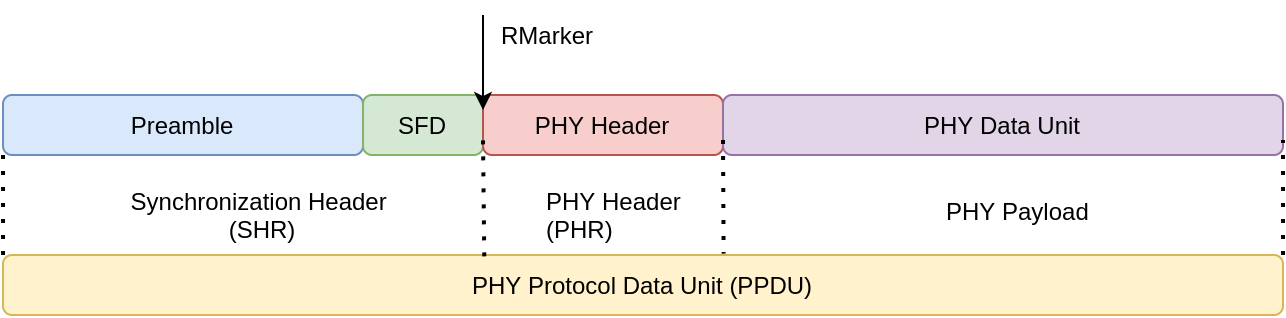
\includegraphics[scale=0.3]{802_15_4_physical.png}
    \end{center}
    \caption{802.15.4 RMarker}
    \label{fig:802_15_4_rmarker}
\end{figure}

\section{Layered architecture}
The ranging system is implemented follow 3 layers model as shown in figure \ref{fig:ranging_layered_architecture}. 
\begin{itemize}
    \item CCP (Clock Calibration Packet) provides synchronization service for the upper layer. All nodes jointed to the network will be synced each time a new superframe start.
    \item TDMA (Time Division Multiple Access): Each superframe is divided into multiple slots. TDMA layer provides slot service for its upper layer. 
    \item TWR (Two Way Ranging) layer runs ranging session in the time slot provided by TDMA layer.
\end{itemize}

Follow the bottom-up approach, detail description about each layer is provided in following sections.
\begin{figure}[H]
    \begin{center}
        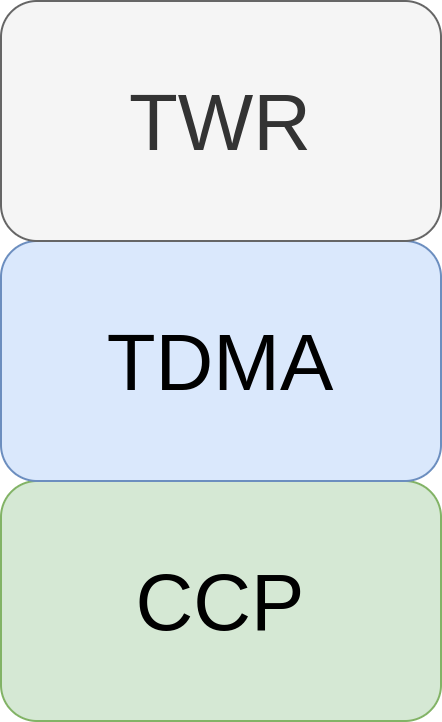
\includegraphics[width=0.2\textwidth]{ranging_layered_architecture}
    \end{center}
    \caption{Ranging layered architecture}
    \label{fig:ranging_layered_architecture}
\end{figure}

\section{Clock calibration packet (CCP)}
The main role clock calibration packet is to provide the superframe synchronization between nodes. 
\subsection{CCP role}
Three CCP roles are defined, allowing nodes to sync with others: Master, Slave, Relay.
\begin{itemize}
    \item \textbf{CCP master}: There is only and only one master node over the network. The master node is the only place where a clock calibration packet is produced. It will produce and transmit the clock calibration packet with the interval defined as a constant in the firmware. My implementation use the value of 100ms for such interval. 
    \item \textbf{CCP slave}: Slave nodes listen for the clock calibration packet to start their internal timer for each superframe.
    \item \textbf{CCP relay}: Relay nodes repeat the clock calibration packet to extend the network physical area. Before repeating the packets, they must do some modification so the receiver can sync with the  master node. There is a constraint in the maximum of repeat level which will be analyzed afterward.
\end{itemize}

To initialize the system, at least one of many nodes must be chosen as a master. The master node will start and control the network and allow other nodes to join and form a network. It is possible to configure more than one node as master, but only one will be active and the others will take the role of slave and/or replay node. A node can take the slave and relay roles at the same time.

\subsection{CCP frame format}
The ccp frame used for synchronization shall be formatted as illustrated in figure \ref{fig:ccp_blink_frame}. The format follow the IEEE 802.15.4-2015 \cite{IEEE_Std_802_15_4_2015} multipurpose frame.
\begin{figure}[H]
    \centering
    \begin{bytefield}[bitwidth=1.1em]{32}
        \bitheader{0-31} \\
        \begin{rightwordgroup}{IEEE \\ header}
            \bitbox{8}{frame control} & 
            \bitbox{8}{sequence number} & \\ 
            \bitbox{32}{extended unique identifier high} \\ 
            \bitbox{32}{extended unique identifier low}
        \end{rightwordgroup} \\
        \begin{rightwordgroup}{Custom\\payload}
            \bitbox{16}{short address} &
            \bitbox{16}{transmission interval high} \\
            \bitbox{32}{transmission interval low} \\
            \bitbox{32}{transmission timestamp high} \\ 
            \bitbox{32}{transmission timestamp low}\\
            \bitbox{8}{repeat count} &
            \bitbox{8}{repeat max}
            \bitbox{16}{epoch to rm us}
        \end{rightwordgroup}
    \end{bytefield}
    \caption{CCP blink frame}
    \label{fig:ccp_blink_frame}
\end{figure}

\subsubsection{Frame Control}
The Frame Control field for the Multipurpose frame are specified in figure \ref{fig:multipurpose_frame_control_field}. Follow standard described in section 7.3.5 of IEEE 802.15.4 \cite{IEEE_Std_802_15_4_2015}, the field is filled up for the purpose of synchronization frame.

\begin{figure}[H]
    \centering
    \begin{bytefield}[bitwidth=5em, bitheight=4em]{8}
        \bitheader{0-7} \\
        \bitbox{3}{Frame Type} &
        \bitbox{1}{Long Frame Control} &
        \bitbox{2}{Destination Addressing Mode} &
        \bitbox{2}{Source Addressing Mode}
        % \bitbox{1}{PAN ID Present} &
        % \bitbox{1}{Security Enabled} &
        % \bitbox{1}{Sequence Number Suppression} &
        % \bitbox{1}{Frame Pending} &
        % \bitbox{2}{Frame Version} &
        % \bitbox{1}{Ack Request} &
        % \bitbox{1}{IE Present}
    \end{bytefield} 
    \caption{Multipurpose frame control field}
    \label{fig:multipurpose_frame_control_field}
\end{figure}
The Frame Type field shall contain the value that indicates a Multipurpose frame as define in IEEE 802.15.4-2015 ($b_2 b_1 b_0 = 101$).

The Long Frame Control field shall be set to \textbf{0} to indicate an MP Short Frame Control field (only bits 0 to 7 make up the Frame Type field).

The Destination Addressing Mode field shall be set to \textbf{0} to indicate PAN ID and destination address fields are not present.

The Source Addressing Mode field shall be set to \textbf{11} to indicate source address field contains an extended address (64-bit Extended Unique Identifier).

For the synchronization purpose, the final value of this field is \textbf{0xC5}.

\subsubsection{Sequence Number}
The Sequence Number field specifies the sequence identifier for the frame.

\subsubsection{Extended Unique Identifier}
Extended Unique Identifier as its name, it is 64-bit unique ID for each device over the globe. DW1000 radio IC takes it from its lot id and part id written by the manufacturer.

\begin{equation}
    \texttt{ euid = ((uint64\_t)lot\_id) << 32 + part\_id}
\end{equation}

\subsubsection{Short address}
The address of sending node in the TDMA network.
\begin{equation}
   \texttt{ short\_address = (uint16\_t)euid \& 0xFFFF}
\end{equation}

\subsubsection{Transmission Interval}
The interval of a superframe, unit of time is a microsecond of DW1000 timer. As previously discussed, 1 microsecond of DW1000 is approximately 512/499.2Mhz. The implementation uses the value of 0x20000, which mean that the transmission interval is:
\begin{equation}
    \texttt{0x20000*(512/499.2Mhz) = 127795.2$\mu$s = 127.7952ms}
\end{equation}

\subsubsection{Transmission Timestamp}
The moment that RMarker is transmitted is the event nominated as the transmit time-stamp. The DW1000 digital transmit circuitry takes note of the system clock counter as the RAW transmit timestamp at the point when it begins sending the PHR. It then adds to this the transmit antenna delay to get the antenna adjusted transmit timestamp.

\subsubsection{Repeat count}
It is the number of non-master nodes that the ccp packet traveled before coming to this node.

\subsubsection{Repeat max}
It is the maximum number of repetition times per packet of ccp.

\subsection{CCP master selection algorithm}

When designing a synchronous system, one of the most fundamental problems is the persistence of the synchronization source. Here, the question is: what will happen if the synchronization source fails, will it stop the entire system from working? This problem is known as the single point of failure (SPOF) problem. SPOFs are undesirable in any system with a goal of high availability or reliability.

To deal with SPOFs, in my implementation, there is no pre-configured node to be master. Instead, all nodes (except for the tag node) can be a master. So, how a node decides itself to be a master or slave? The main idea is the lazy mindset: master is hard work, I will not take it, but if nobody does, I will. Figure \ref{fig:CCP_state_diagram} illustrates this mindset.

\begin{figure}[H]
    \begin{center}
        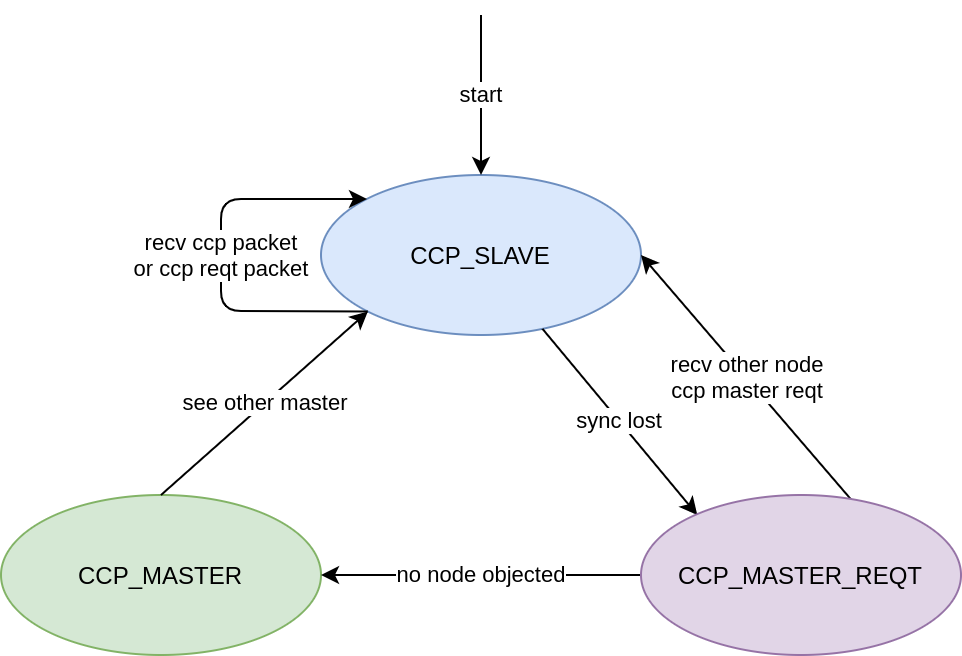
\includegraphics[scale=0.35]{ccp_state_diagram.png}
    \end{center}
    \caption{CCP state transition diagram}
    \label{fig:CCP_state_diagram}
\end{figure}

As shown in figure \ref{fig:CCP_state_diagram}, all node will start with ccp slave role. If there is already a master node, a just-powered-on node will receive ccp packets from the master node and remain in the slave state. If there is no master node, after its internal counter reaches a conditional random thresh hold, it will turn into the master request state. It now sends ccp request packets and listens for objection for a while. If no node object, the new state is ccp master. If it receives any ccp packet or ccp request packet in the master or master request state, it will immediately turn into the slave state as it is lazy.

Figure \ref{fig:ccp_slave_flow_chart}, \ref{fig:ccp_master_reqt_flow_chart} and \ref{fig:ccp_master_flow_chart} are simplified flowcharts used for implementing each state.

Figure \ref{fig:ccp_slave_flow_chart} is the flow chart for CCP\_SLAVE state. In this state, rx\_timeout\_counter variable is used to timeout the slave and turn it into the CCP\_MASTER\_REQT state.
This variable is also checked for each RX timer callback, if it is not equal to 0, which means that there is a timeout event before, it is necessary to listen immediately to increase the chance of receiving the next ccp packet. If the variable equal to 0, the MCU will schedule the radio IC to receive the frame at a calculated moment. If a ccp packet is successfully received, MCU will schedule the next wake up to receive the next ccp packet based on the ccp packet it just received. 

Figure \ref{fig:ccp_master_reqt_flow_chart} is the flow chart for
CCP\_MASTER\_REQT state. In this state, a node will periodically send the ccp request packet. If no node protests by sending another cpp packet or ccp request packet, the variable master\_reqt\_state is used to timeout the CCP\_MASTER\_REQT state and turn the node into the master state.

Figure \ref{fig:ccp_master_flow_chart} is the flow chart for CCP\_MASTER state. A node enters this state by scheduling a TX timer and waiting for its timeout. This timer will wake up the CPU to schedule the radio IC for transmitting ccp packet at a calculated moment. The listen stage here is for the demonstration purpose only. In fact, the ccp packet does not listen in the master state. Instead, the ccp implementation act as an observer to analyze any packet received in the superframe internal interval. Packets must be received by listen commands of higher layers.

\begin{figure}[H]
    \begin{center}
        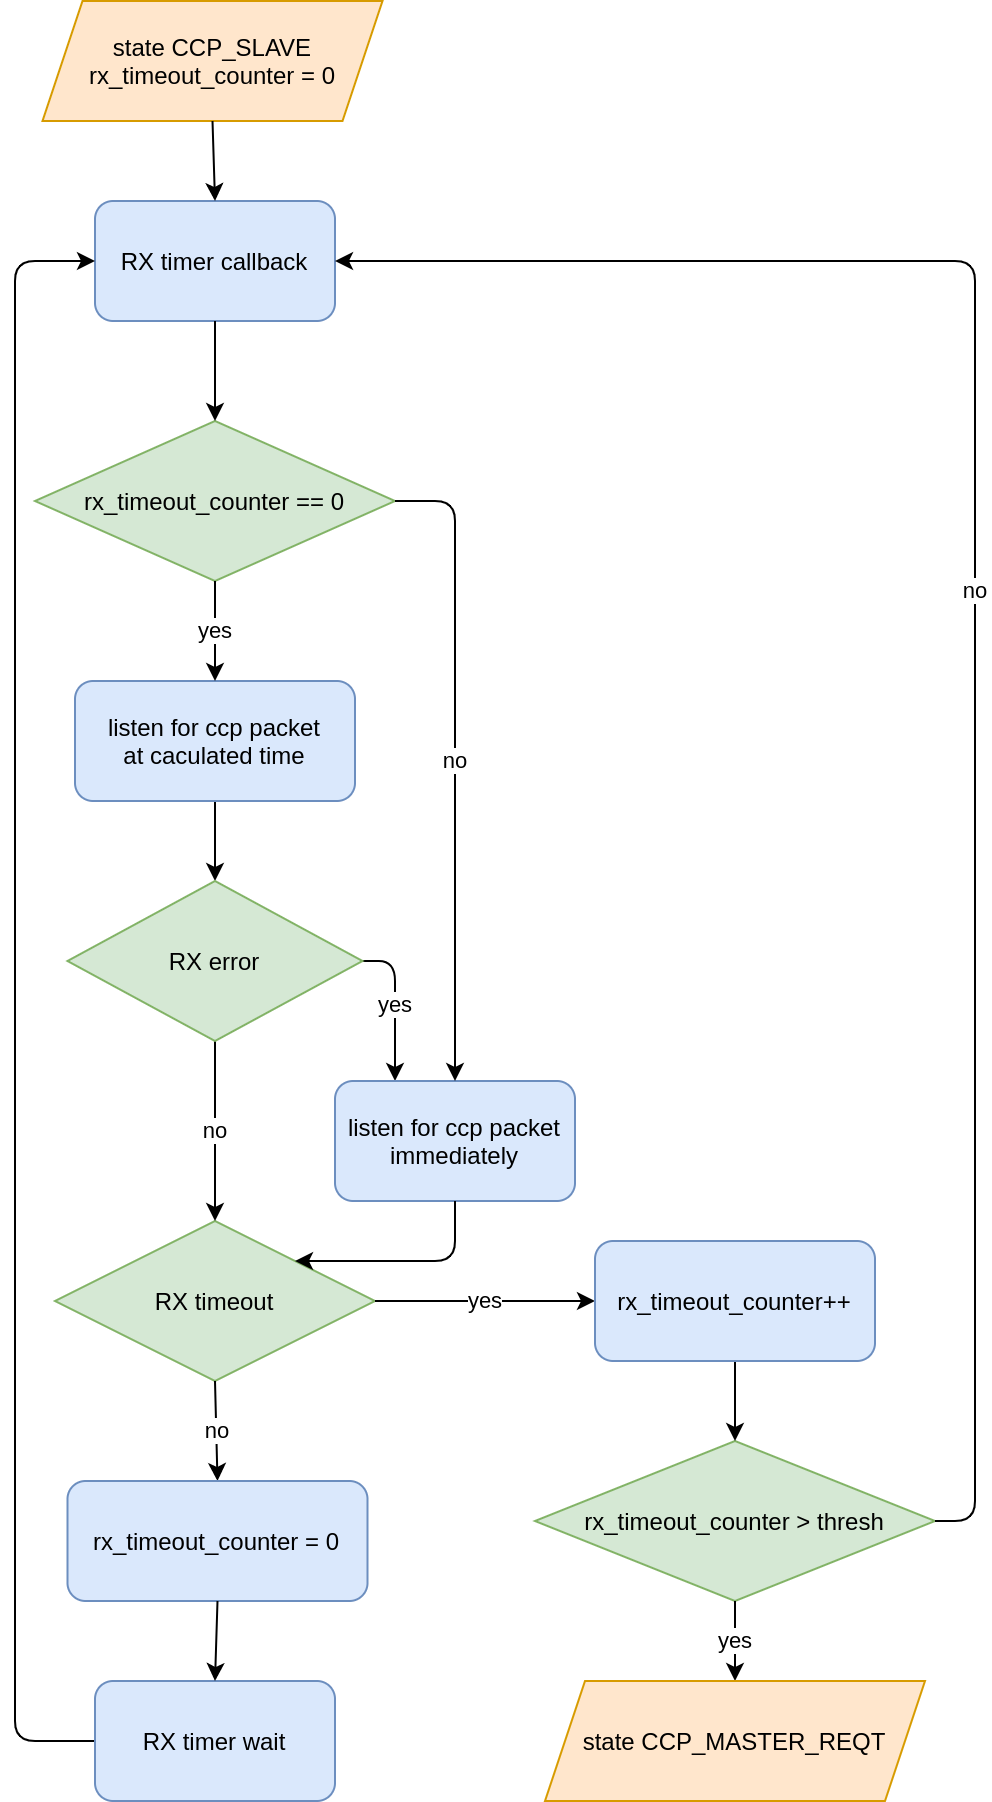
\includegraphics[scale=0.35]{ccp_slave_flow_chart.png}
    \end{center}
    \caption{CCP slave flow chart}
    \label{fig:ccp_slave_flow_chart}
\end{figure}

% \begin{figure}[H]
%     \begin{center}
%         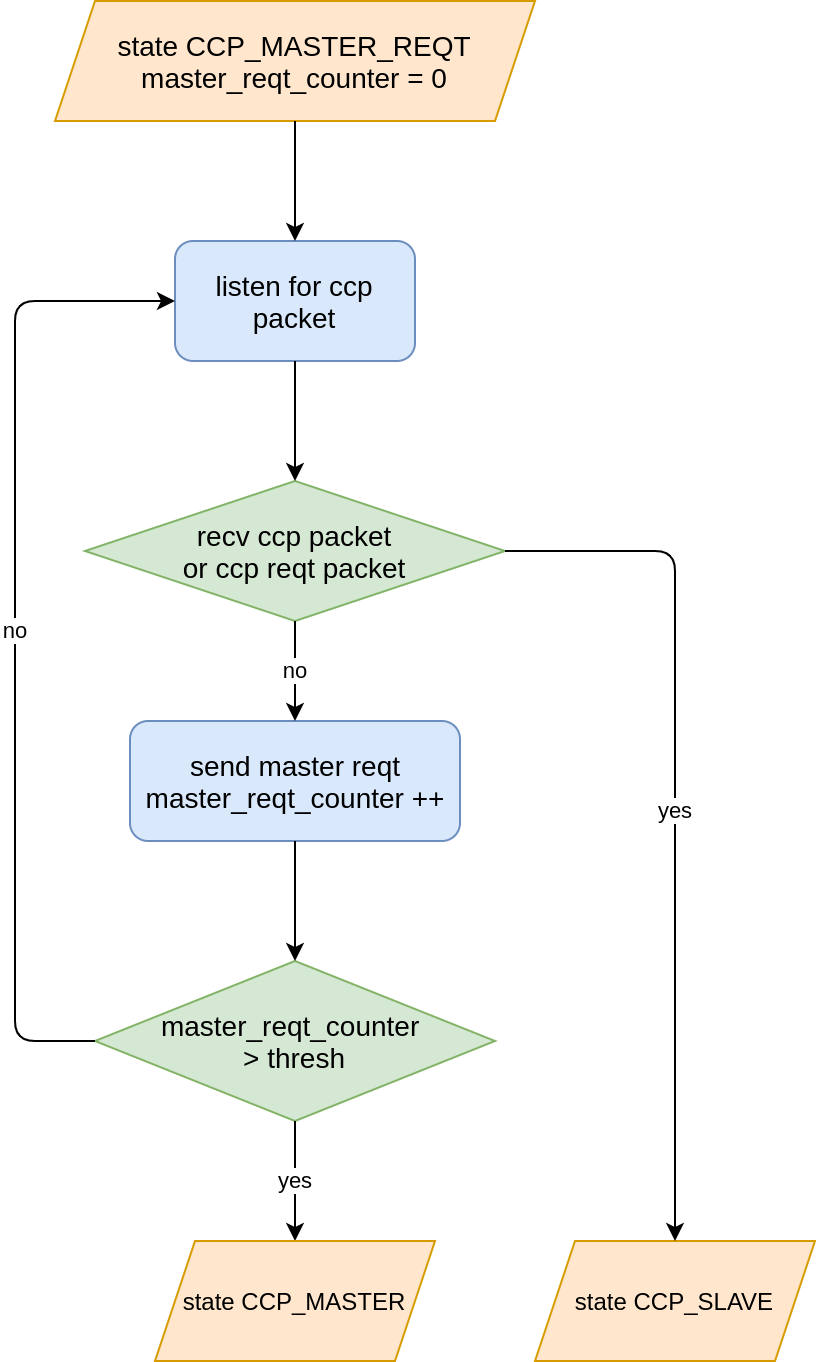
\includegraphics[scale=0.35]{ccp_master_reqt_flow_chart.png}
%     \end{center}
%     \caption{CCP master request flow chart}
%     \label{fig:ccp_master_reqt_flow_chart}
% \end{figure}

% \begin{figure}[H]
%     \begin{center}
%         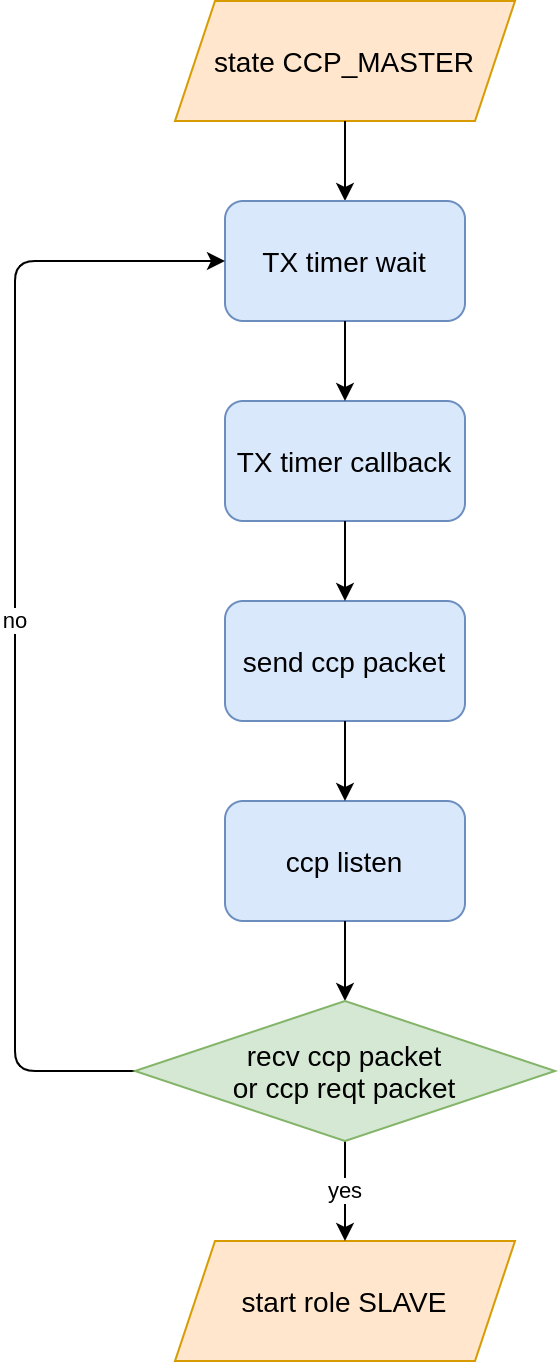
\includegraphics[scale=0.35]{ccp_master_flow_chart.png}
%     \end{center}
%     \caption{CCP master flow chart}
%     \label{fig:ccp_master_flow_chart}
% \end{figure}

\begin{figure}
    \centering
    \begin{subfigure}[b]{0.47\textwidth}
        \begin{center}
            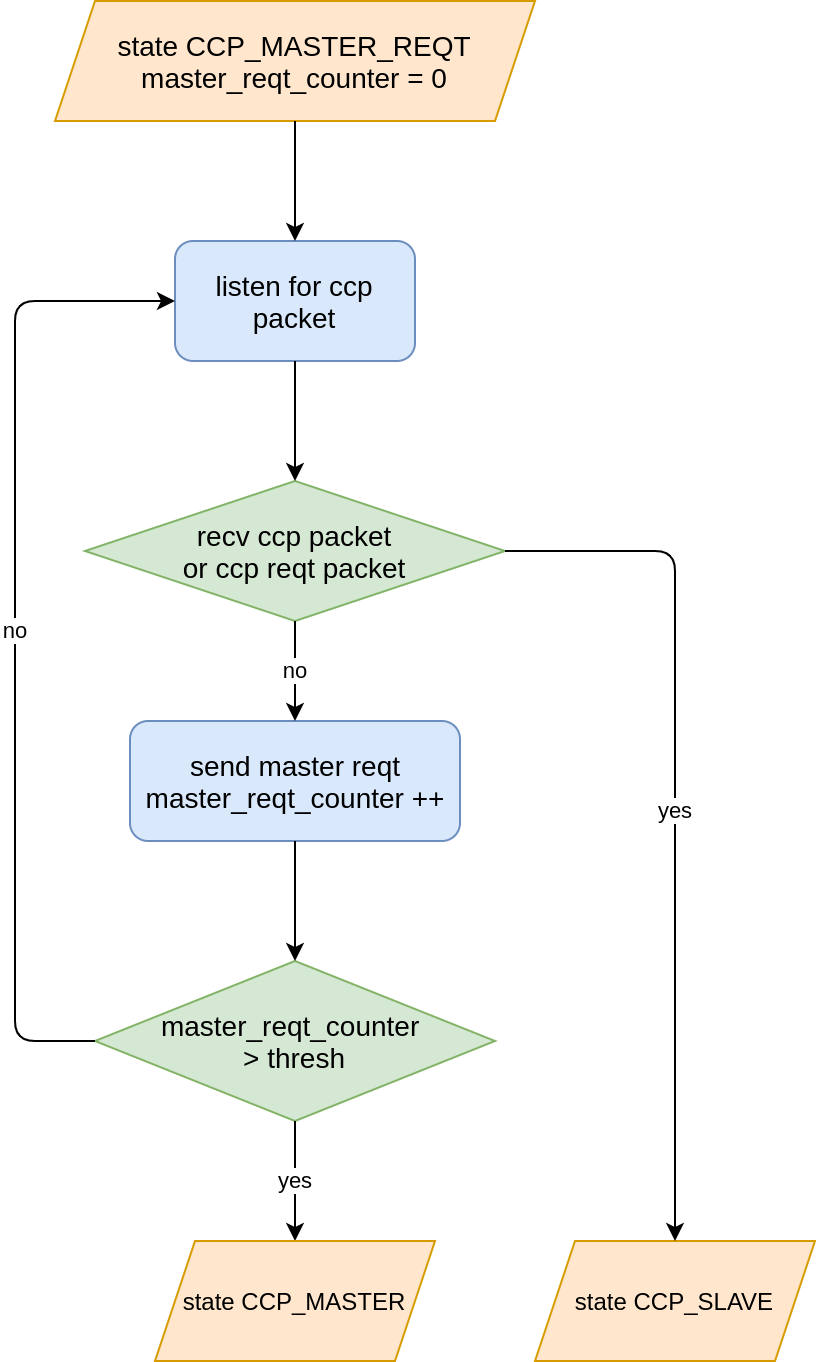
\includegraphics[scale=0.3]{ccp_master_reqt_flow_chart.png}
        \end{center}
        \caption{CCP master request flow chart}
        \label{fig:ccp_master_reqt_flow_chart}
    \end{subfigure}
    \hfill
    \begin{subfigure}[b]{0.47\textwidth}
        \begin{center}
            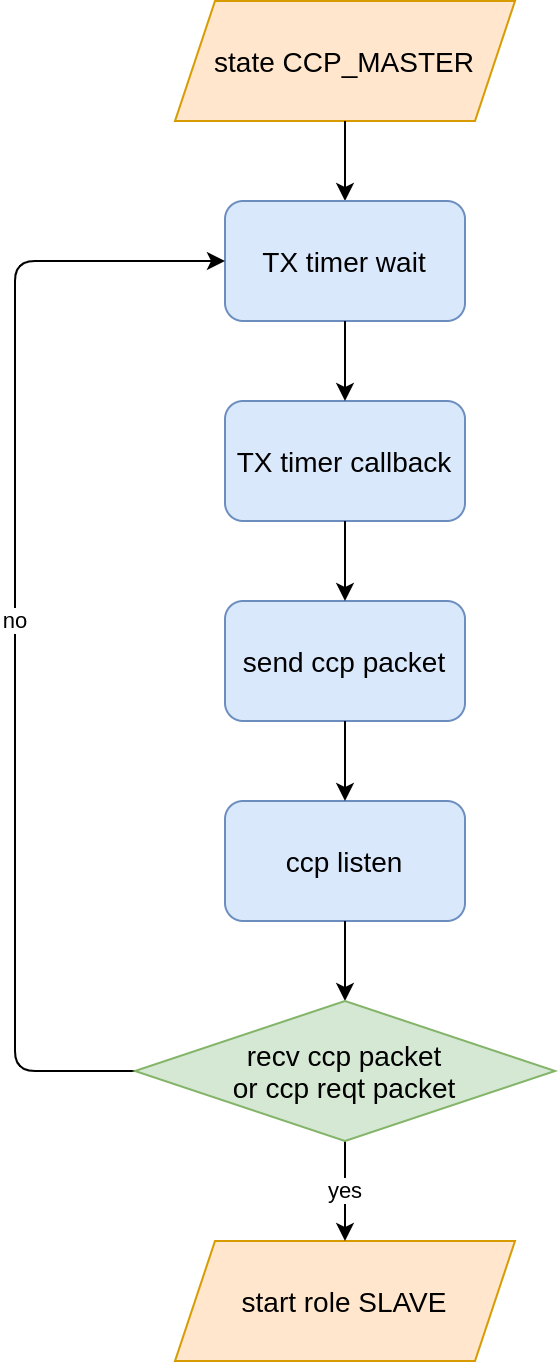
\includegraphics[scale=0.3]{ccp_master_flow_chart.png}
        \end{center}
        \caption{CCP master flow chart}
        \label{fig:ccp_master_flow_chart}
    \end{subfigure}
    \caption{CCP master and master request flow chart}
\end{figure}

% \begin{figure}
%     \begin{subfigure}[b]{0.45\textwidth}
%         \begin{center}
%         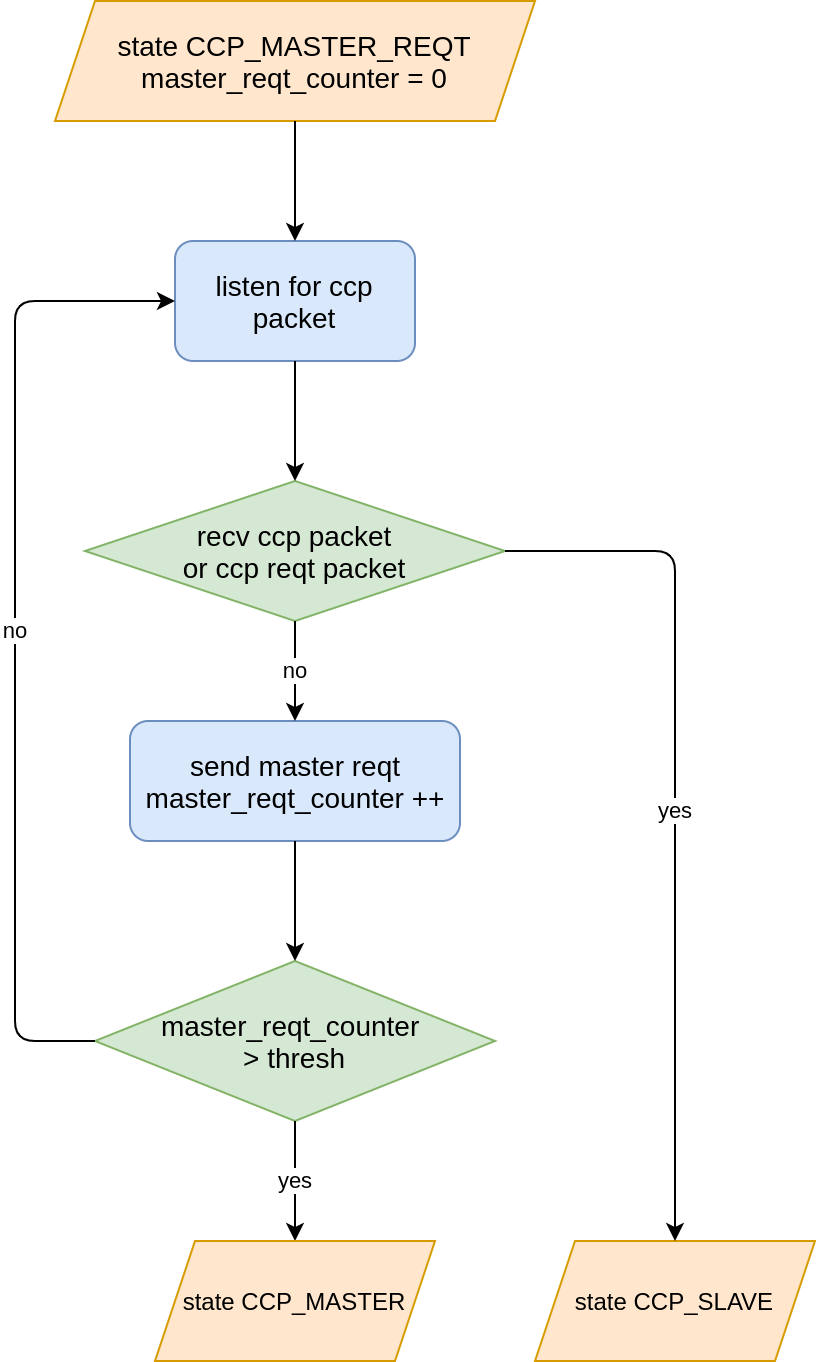
\includegraphics[scale=0.25]{ccp_master_reqt_flow_chart.png}
%     \end{center}
%         \caption{CCP master request flow chart}
%         \label{fig:ccp_master_reqt_flow_chart}
%     \end{subfigure}
%     %
%     \begin{subfigure}[b]{0.45\textwidth}
%         \begin{center}
%     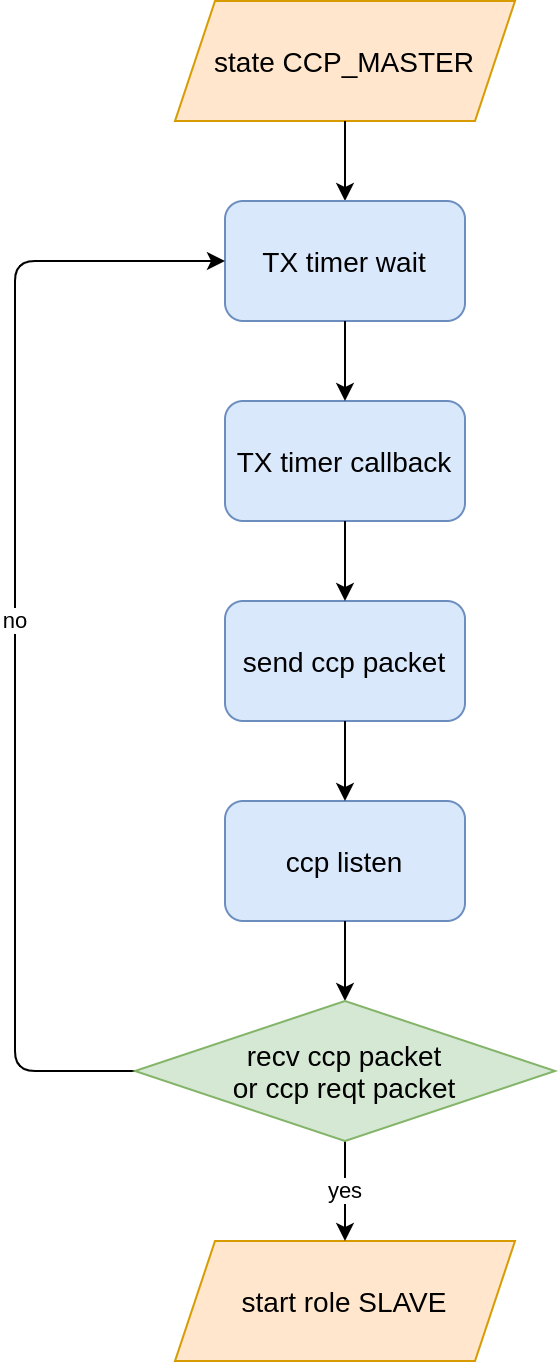
\includegraphics[scale=0.3]{ccp_master_flow_chart.png}
% \end{center}
%     \caption{CCP master flow chart}
%     \label{fig:ccp_master_flow_chart}
%     \end{subfigure}
%   \end{figure}

\subsection{CCP implementation}
This section discusses detailed timing problems related to CCP. Before starting, some fundamental concepts should be defined and accepted:
\begin{itemize}
    \item Master epoch $ep_m$: Packet timestamp referenced to CCP master device timing system.
    \item Local epoch $ep_l$: Packet timestamp referenced to CCP slave device timing system.
    \item Os epoch $ep_o$: Packet timestamp referenced to CCP master or slave host timing system.
    \item Period $\tau$: The interval of a superframe.
    \item $t^k_{m}$: Timestamp for $k$th frame in device timing system of master node.
    \item $t^k_{l}$: Timestamp for $k$th frame in device timing system of local node.
    \item $t_h$: Current host time (in host timing system).
    \item $t_d$: Current device time (in device timing system).
    \item $f_{d2h}$: A linear function for converting the device time to host time as explained in \ref{subsec:timing_system_subsection}
    \item $T_{latency}$: OS latency is the interval for OS to process before sending.
    \item $T_{SHR}$: The interval between an epoch and a RMarker which is also the duration of SHR as shown in figure \ref{fig:ccp_epoch_and_rmarker}.
    \item $T_{PHY}$: Total duration of PHY Header and PHY data unit.
\end{itemize}
\begin{figure}[H]
    \begin{center}
        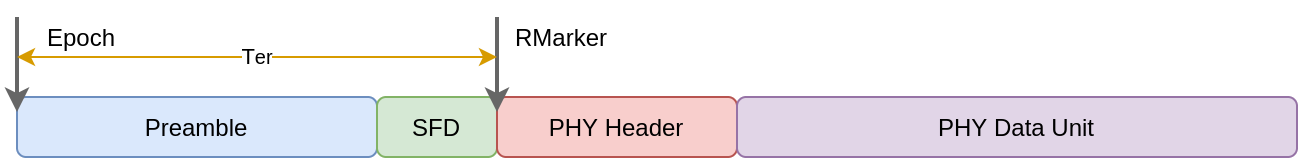
\includegraphics[scale=0.35]{ccp_epoch_and_rmarker.png}
    \end{center}
    \caption{CCP epoch and RMarker}
    \label{fig:ccp_epoch_and_rmarker}
\end{figure}

\subsubsection{Calculate the SHR (Preamble + SFD) duration $T_{SHR}$}
\begin{equation}
    T_{SHR} = T_{psym}(n_{sync} + n_{sfd})
\end{equation}
With:
\begin{itemize}
    \item $T_{psym} = 1.0176282 \mu s$: Preamble symbols duration for mean PRF (Pulse Repetition Frequency) of 62.89Mhz
    \item $n_{sync} = 128 $: Number of symbols in preamble sequence
    \item $n_{sfd}$ = 8: Number of symbols in start of frame delimiter
\end{itemize}
All of these parameters can be taken from IEEE 802.15.4-2015 standard \cite{IEEE_Std_802_15_4_2015}, table 16-5.

\subsubsection{Calculate the PHY duration $T_{PHY}$}
Since it is necessary to add 48 parity bits for every 330 bits in the data payload (including CRC), the total number of parity bits is:
\begin{equation}
    n_{parity} = 48 + 48\frac{8(n_{len}+2)}{330}
\end{equation}
With $n_{len}$ is size of PHY payload in byte.
The total number of PHY payload is:
\begin{equation}
    n_{phy-payload} = 8*(n_{len}+2) + n_{parity}
\end{equation}
Finally, the duration for PHY is:
\begin{equation}
    T_{PHY} = T_{bsym} * n_{phy-header} + T_{dsym} * n_{phy-payload}
\end{equation}
Where:
\begin{itemize}
    \item $T_{bsym} = 1.0256410 \mu s$: Baserate symbols duration 850khz
    \item $T_{dsym} = 0.1282051 \mu s$: Datarate symbols duration (usec) 6.81Mhz
    \item $n_{phy-header} = 21$: Number of symbols in phy header
\end{itemize}
These parameters can be taken from IEEE 802.15.4-2015 standard \cite{IEEE_Std_802_15_4_2015}, table 16-3.

\subsubsection{CCP timing for master node}

The CCP packet is sent with timestamp calculated from previous frame:
\begin{equation}
    t^k_m = t^{k-1}_m + \tau
\end{equation}

Each time the CCP master node complete to send a CCP packet, a TX event is called for re-calculating $ep_m$, $ep_l$ and $ep_o$ using the following formulas:
\begin{equation}
    ep_m = ep_l = t^k_m - T_{SHR}
\end{equation}

$ep_o$ is calculated form current host time:
\begin{equation}
    ep_o = t_h - f_{d2h}(t_d - t^k_m) - T_{SHR}
\end{equation}
where $f_{d2h}$ is a function to convert from device timing system to host timing system.

After sending the CCP packet, the MCU will schedule for the next wake up at:
\begin{equation}
    t_{wake up} = ep_o + \tau - T_{latency}
\end{equation}

\begin{figure}[H]
    \begin{center}
        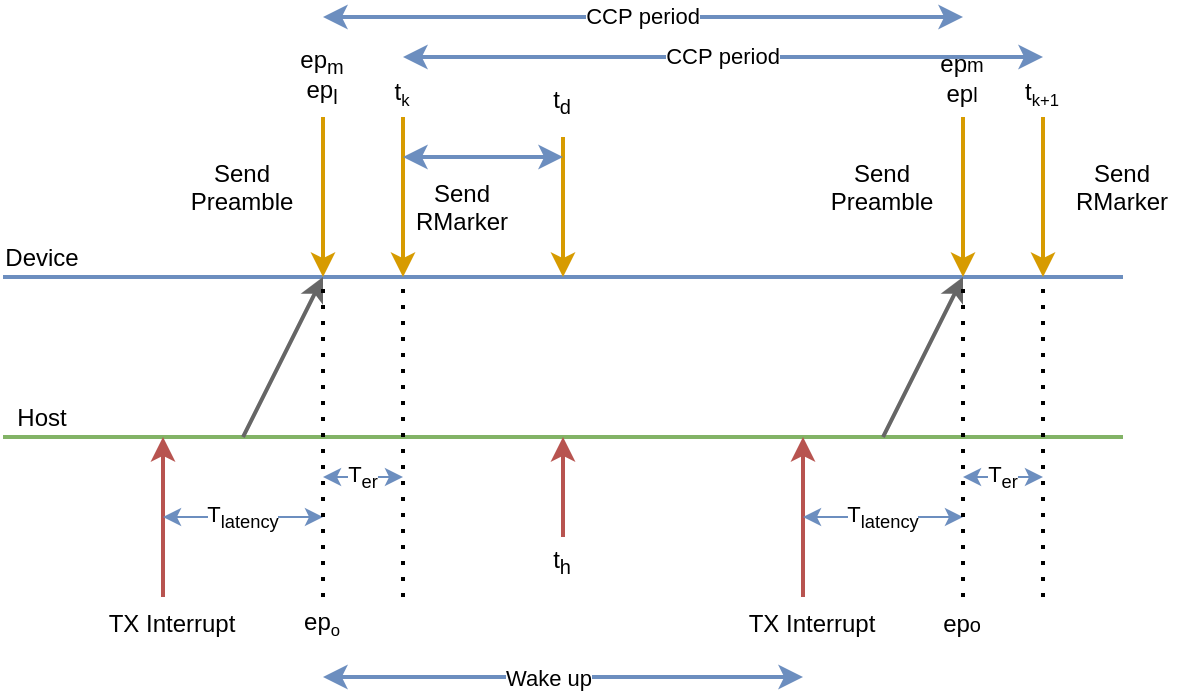
\includegraphics[width=1\textwidth]{ccp_timing_for_master_node.png}
    \end{center}
    \caption{CCP master timing}
    \label{fig:interupt_latency_master}
\end{figure}

\subsubsection{CCP timing for slave node}

Each time the CCP slave node complete to receive a CCP packet, a RX event is called for re-calculating $ep_m$, $ep_l$ and $ep_o$ using the following formulas:

$ep_m$ is calculated from timestamp field $t^k_m$ of received frame:
\begin{equation}
    ep_m = t^k_m - T_{SHR}
\end{equation}

$ep_l$ is calculated from current device time:
\begin{equation}
ep_l = t^k_l - T_{SHR}
\end{equation}

$ep_o$ is calculated form current host time:
\begin{equation}
    ep_o = t_h - f_{d2h}(t_d - t^k_l) - T_{SHR}
\end{equation}

After processing the CCP packet, the MCU will schedule for the next wake up at:
\begin{equation}
    t_{wake up} = ep_o + \tau - T_{latency}
\end{equation}
% To make it easier for calibrating $T_{latency}$, the cpp frame duration and rx stable interval is taken into account:
% \begin{equation}
%     t_{wake up} -= t_{ccp-frame} + t_{wake up}
% \end{equation}
% With:
% \begin{itemize}
%     \item $t_{ccp-frame} = T_{SHR} + T_{PHY}$: The duration of physical ccp frame.
%     \item $t_{rx-stable} = 6 \mu s$: The interval for a frame  to be stable.
% \end{itemize}

\begin{figure}[H]
    \begin{center}
        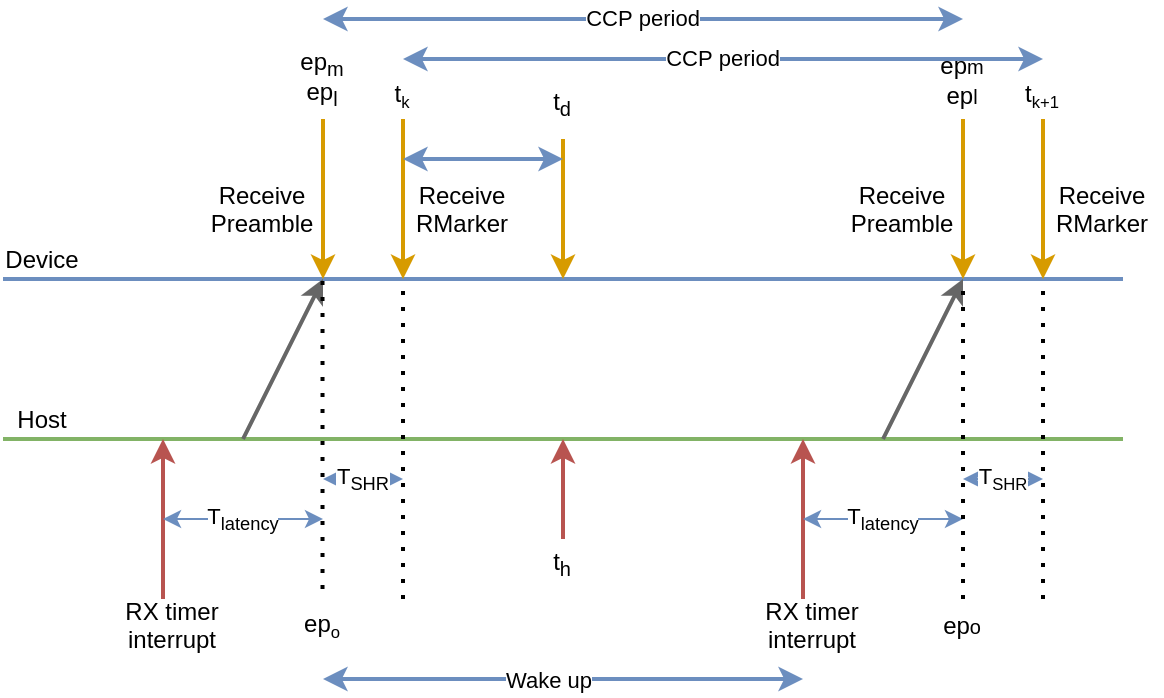
\includegraphics[width=1\textwidth]{ccp_timing_for_slave_node.png}
    \end{center}
    \caption{CCP master timing}
    \label{fig:ccp_timing_for_slave_node}
\end{figure}

\subsubsection{Cascade relay of ccp packet}
% \subsubsection{Repeat CCP packet}
% \begin{figure}[H]
%     \begin{center}
%         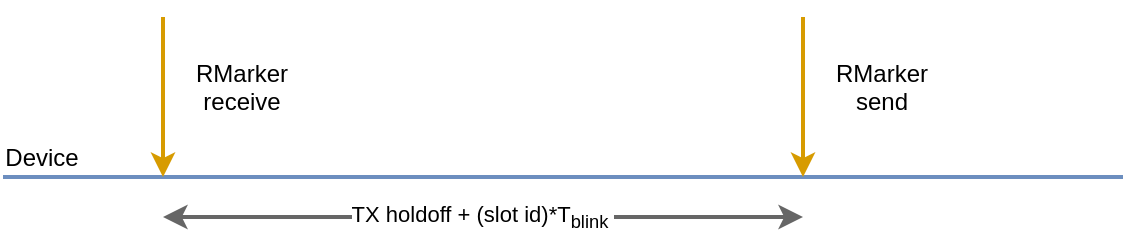
\includegraphics[scale=0.35]{ccp_repeat.png}
%     \end{center}
%     \caption{CCP Repeat}
%     \label{fig:ccp_repeat}
% \end{figure}
When a node receives a CCP packet and want to repeat it, it have to hold the CCP packet for $T_{hold-off}$ before re-transmitting.
\begin{equation}
    T_{hold-off} = n_{repeat}*T_{hold-off-conf} + i_{slot}*T_{ccp}
\end{equation}
Where:
\begin{itemize}
    \item $n_{repeat}$ is the number of times that packet has been repeated plus 1
    \item $T_{hold-off-conf}$ is a configurable parameter for holding the CCP packet before re-transmitting it
    \item $i_{slot}$ is the slot index of the node in the TDMA system as described in the following section
    \item  $T_{ccp}$ is the duration of a CCP packet
\end{itemize}

The CCP packet is repeated with timestamp calculated from equation \ref{eqn:cpp_repeat_timestamp}.
\begin{equation}
    t^k_m = t_{k-repeat} = t_k + T_{delay}
    \label{eqn:cpp_repeat_timestamp}
\end{equation}

The hold off delay of a repeated ccp packet takes into account of transition interval or CCP period as shown in equation \ref{eqn:ccp_hold_off_vs_ccp_period}.
\begin{equation}
    \tau_{new} = \tau - T_{hold-off}
    \label{eqn:ccp_hold_off_vs_ccp_period}
\end{equation}

\section{Time Division Multiple Access (TDMA)}
The fundamental role of the TDMA layer is to give a notification to its upper layer when it is the time to run the service. To archive this, a node must firstly ask for getting an appropriate and available slot from jointed nodes.

\subsection{TDMA role}
In the TDMA layer, a jointed node must take one of two roles: Anchor or Tag.
\begin{itemize}
    \item TDMA Anchor: A node taking the role as an anchor must be fixed and broadcast its pre-configured location information to others.
    \item TDMA Tag: TDMA tag node is the mobile node needed to be located in the coordinate of anchors.
\end{itemize}

\subsection{TDMA slot}
The superframe is divided into multiple slots as shown in figure \ref{fig:tdma_slot}.
\begin{figure}[ht]
    \begin{center}
        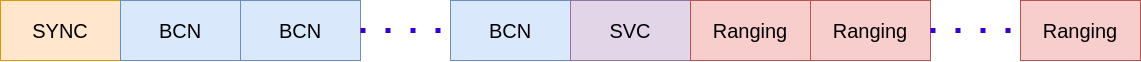
\includegraphics[scale=0.4]{tdma_slot.png}
    \end{center}
    \caption{TDMA slot}
    \label{fig:tdma_slot}
\end{figure}

\subsubsection{Synchronization slot (SYNC slot)}
In the SYNC slot interval, a master node produces and transmits the clock calibration packet. Relay nodes also repeat the clock calibration packet in this interval too.
\subsubsection{Beacon slot (BCN slot)}
An anchor node will broadcast its location and slot map information in its BCN slot. It is allowed for a jointed anchor to skip some superframes as long as it does not exceed a certain value. Other anchor nodes consider a node has left the network when they do not see any BCN message from such node for a number of superframes. The implementation uses the value of 10 for this purpose.
\subsubsection{SVC slot (Service slots)}
When a node wants to joint the network as a tag or anchor, it has to send its joint request in an SVC slot. The request is broadcasted and responded by all jointed anchors in their next assigned BCN slot.
\subsubsection{Ranging slot}
A jointed tag initiates the range request in its assigned ranging slot. During the remaining interval, it also listens for the response from anchors to calculate to ToF (Time of Flight).

\subsubsection{TDMA timing}
Each software timer is assigned for each tdma slot. Such timers will expire and raise an event to the upper layer as a service. Timer duration is calculated using the equation \ref{eqn:tdma_timing} as shown in figure \ref{fig:tdma_timing}.
\begin{equation}
    t = ep_o + d_{slot}*i_{slot} - T_{latency}
    \label{eqn:tdma_timing}
\end{equation}
With: 
\begin{itemize}
    \item $t$: The moment at which the timer expire referred to the host timing system.
    \item $d_{slot} = \frac{\tau}{n_{slot}}$: The duration of a slot which is equal to the duration of a superframe divide by the total number of slots.
    \item $T_{latency}$: The OS latency
\end{itemize}

\begin{figure}[H]
    \begin{center}
        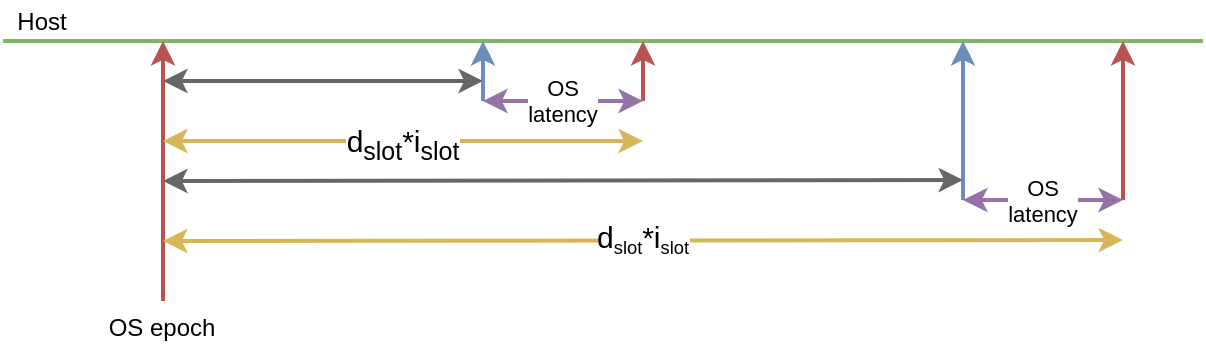
\includegraphics[width=1\textwidth]{tdma_timing.png}
    \end{center}
    \caption{TDMA timing}
    \label{fig:tdma_timing}
\end{figure}


\subsection{TDMA frame format}
All TDMA frames consist two fields:
\begin{itemize}
    \item IEEE fame header which conforms the 802.15.4-2015 standard.
    \item Payload field which may contain more than one message. 
\end{itemize}

\begin{figure}[H]
    \centering
    \begin{bytefield}[bitwidth=1.1em]{32}
        \bitheader{0-31} \\
        \begin{rightwordgroup}{IEEE \\ frame \\ header}
            \bitbox{16}{frame control} & 
            \bitbox{8}{sequence number} \\ 
            \bitbox{16}{pand id} \\
            \bitbox{16}{dst address} &
            \bitbox{16}{src address} 
        \end{rightwordgroup} \\
        \wordbox[tlr]{1}{payload} \\
        \wordbox[blr]{1}{$\cdots$}
    \end{bytefield}
    \caption{TDMA frame}
    \label{fig:tdma_frame}
\end{figure}

\subsubsection{Frame Control}
The Frame Control field for the standard Data frame are specified in figure \ref{fig:function_control_for_standard_data_frame}.

\begin{figure}[H]
    \centering
    \begin{bytefield}[bitwidth=2.6em, bitheight=6em]{16}
        \bitheader{0-15} \\
        \bitbox{3}{Frame Type} &
        \bitbox{3}{} &
        \bitbox{1}{PAN ID Compression} &
        \bitbox{3}{} &
        \bitbox{2}{Destination Addressing Mode} &
        \bitbox{2}{} &
        \bitbox{2}{Source Addressing Mode}
    \end{bytefield}
    \caption{Function Control for stand Data Frame}
    \label{fig:function_control_for_standard_data_frame}
\end{figure}
The Frame Type field shall be set as $b_2 b_1 b_0 = 001$ for data frame.

The PAN ID Compression field is used to indicate the presence of the PAN ID field. As both destination and source addressing information is present, the MAC sub-layer shall compare the destination and source PAN identifiers and see the PAN IDs are identical, the PAN ID Compression field should be set to 1 and the Source PAN ID field is omitted from the transmitted frame. 

The Destination Addressing Mode field shall be set to  $b_1 b_0 = 10$ as the destination address field contains a short address (16 bit).

The Source Addressing Mode field shall be set to  $b_1 b_0 = 10$ as the source address field contains a short address (16 bit).

The final value for the frame control field is: \textbf{0x8841}
\subsubsection{Sequence Number}
The Sequence Number field specifies the sequence identifier for the frame

\subsubsection{Pan ID}
The Destination PAN ID field is an unsigned integer that specifies the unique PAN ID of the intended recipient of the frame. 

\subsubsection{Dst Address}
The Destination Address field with a length specified in the Destination Addressing Mode field of the Frame Control field specifies the address of the intended recipient of the frame.

\subsubsection{Src Address}
The Source Address field specifies the address of the originator of the frame. As the Source Addressing Mode field is nonzero, this field is included in the MAC frame.

\subsubsection{Payload}
The Frame Payload field contains information specific to individual frame types. Each message in payload have TLV (type-length-value) format as shown in figure \ref{fig:tdma_frame_payload}.

TLV format, the Type-Length-Value encoding, is used for data exchanging between nodes. Data in TLV format always begins with the type byte, followed by the length byte, and then followed by a variable number of value bytes as specified by the length byte.

\begin{figure}[ht]
    \centering
    \begin{bytefield}[bitwidth=1.1em]{32}
        \bitheader{0-15}\\
        \bitbox{8}{type} & 
        \bitbox{8}{length} & 
        \bitbox{16}{value}
    \end{bytefield}
    \caption{TDMA frame payload}
    \label{fig:tdma_frame_payload}
\end{figure}

Currently, three message types are defined: \textbf{Slot request/response}, \textbf{Location}, \textbf{Slot map}. The value of these message type are illustrated in figure \ref{fig:slot_request_response_message}, \ref{fig:location_value}, \ref{fig:slot_map_message}.

\subsubsection{Slot request/response message}
\begin{figure}[H]
    \centering
    \begin{bytefield}[bitwidth=2em]{16}
        \bitheader{0-15} \\
        \bitbox{8}{slot} &
        \bitbox{8}{slot request/response}
    \end{bytefield}
    \caption{Slot request/response message}
    \label{fig:slot_request_response_message}
\end{figure}

\subsubsection{Location message}
\begin{figure}[H]
    \centering
    \begin{bytefield}[bitwidth=1.1em]{32}
        \bitheader{0-31} \\
        \bitbox{8}{slot} \\
        \bitbox{32}{location x} \\
        \bitbox{32}{location y} \\ 
        \bitbox{32}{location z}
    \end{bytefield}
    \caption{Location message value}
    \label{fig:location_value}
\end{figure}

\subsubsection{Slot map message}
\begin{figure}[H]
    \centering
    \begin{bytefield}[bitwidth=1.1em]{32}
        \bitheader{0-31} \\
        \bitbox{8}{slot} \\
        \bitbox{32}{slot map high} \\
        \bitbox{32}{slot map low}
    \end{bytefield}
    \caption{Slot map message}
    \label{fig:slot_map_message}
\end{figure}

\subsection{Network management algorithm}

\subsubsection{State diagram}
The TDMA state diagram is shown in figure \ref{fig:tdma_state_diagram}. 
The master node is the initiator of the network. It has to be an anchor and occupy BCN slot 1. Since there is no jointed node before, the master node does not need to ask others. Hence, after ccp layer provides first synchronization, all nodes begin with REQT state except for the master node. 

\begin{figure}[H]
    \begin{center}
        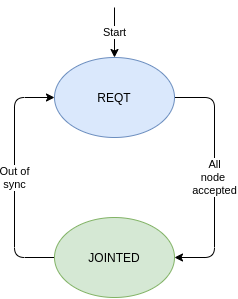
\includegraphics[width=0.4\textwidth]{tdma_state_diagram.png}
    \end{center}
    \caption{TDMA state diagram}
    \label{fig:tdma_state_diagram}
\end{figure}

\subsubsection{REQT state flow chart}
The REQT state implementation is illustrated in the flow chart \ref{fig:REQT_state_flowchart}. The system is likely to be an  organization that a new member can only joint if all jointed members accept it. As all jointed anchors have a list of occupied slots, this joint mechanism makes sure that one anchor will never see more than one anchor in a time slot. It also makes a slot re-usable at different regions.

In a BCN slot, a node listens for a BCN message, if it sees a new anchor, it will add that node to its anchor list and process the BCN message. If it received a slot-accept message, it will check if all node in its anchor list has accepted for its slot, if it is true, that node will enter the JOINT state.

In an SVC slot, a node sends a joint-request message to all nodes in its anchor list.


\subsubsection{JOINTED state flow chart}
The JOINTED state implementation is illustrated in the follow chart \ref{fig:JOINTED_state_flowchart}.

The SYNC slot is used to timeout and remove a node from the node list.

In its BCN slot, a jointed anchor sends a beacon message to broadcast its state. If it is its BCN slot, such node will listen for BCN message to reset the timeout timer of each anchor and update anchor information based on the message received. An anchor also responds to slot request message in its slot.

In the SVC slot, jointed anchors will listen for a joint-request message.

In a Ranging slot, jointed anchors will listen for a range-request message.

\begin{figure}[H]
    \begin{center}
        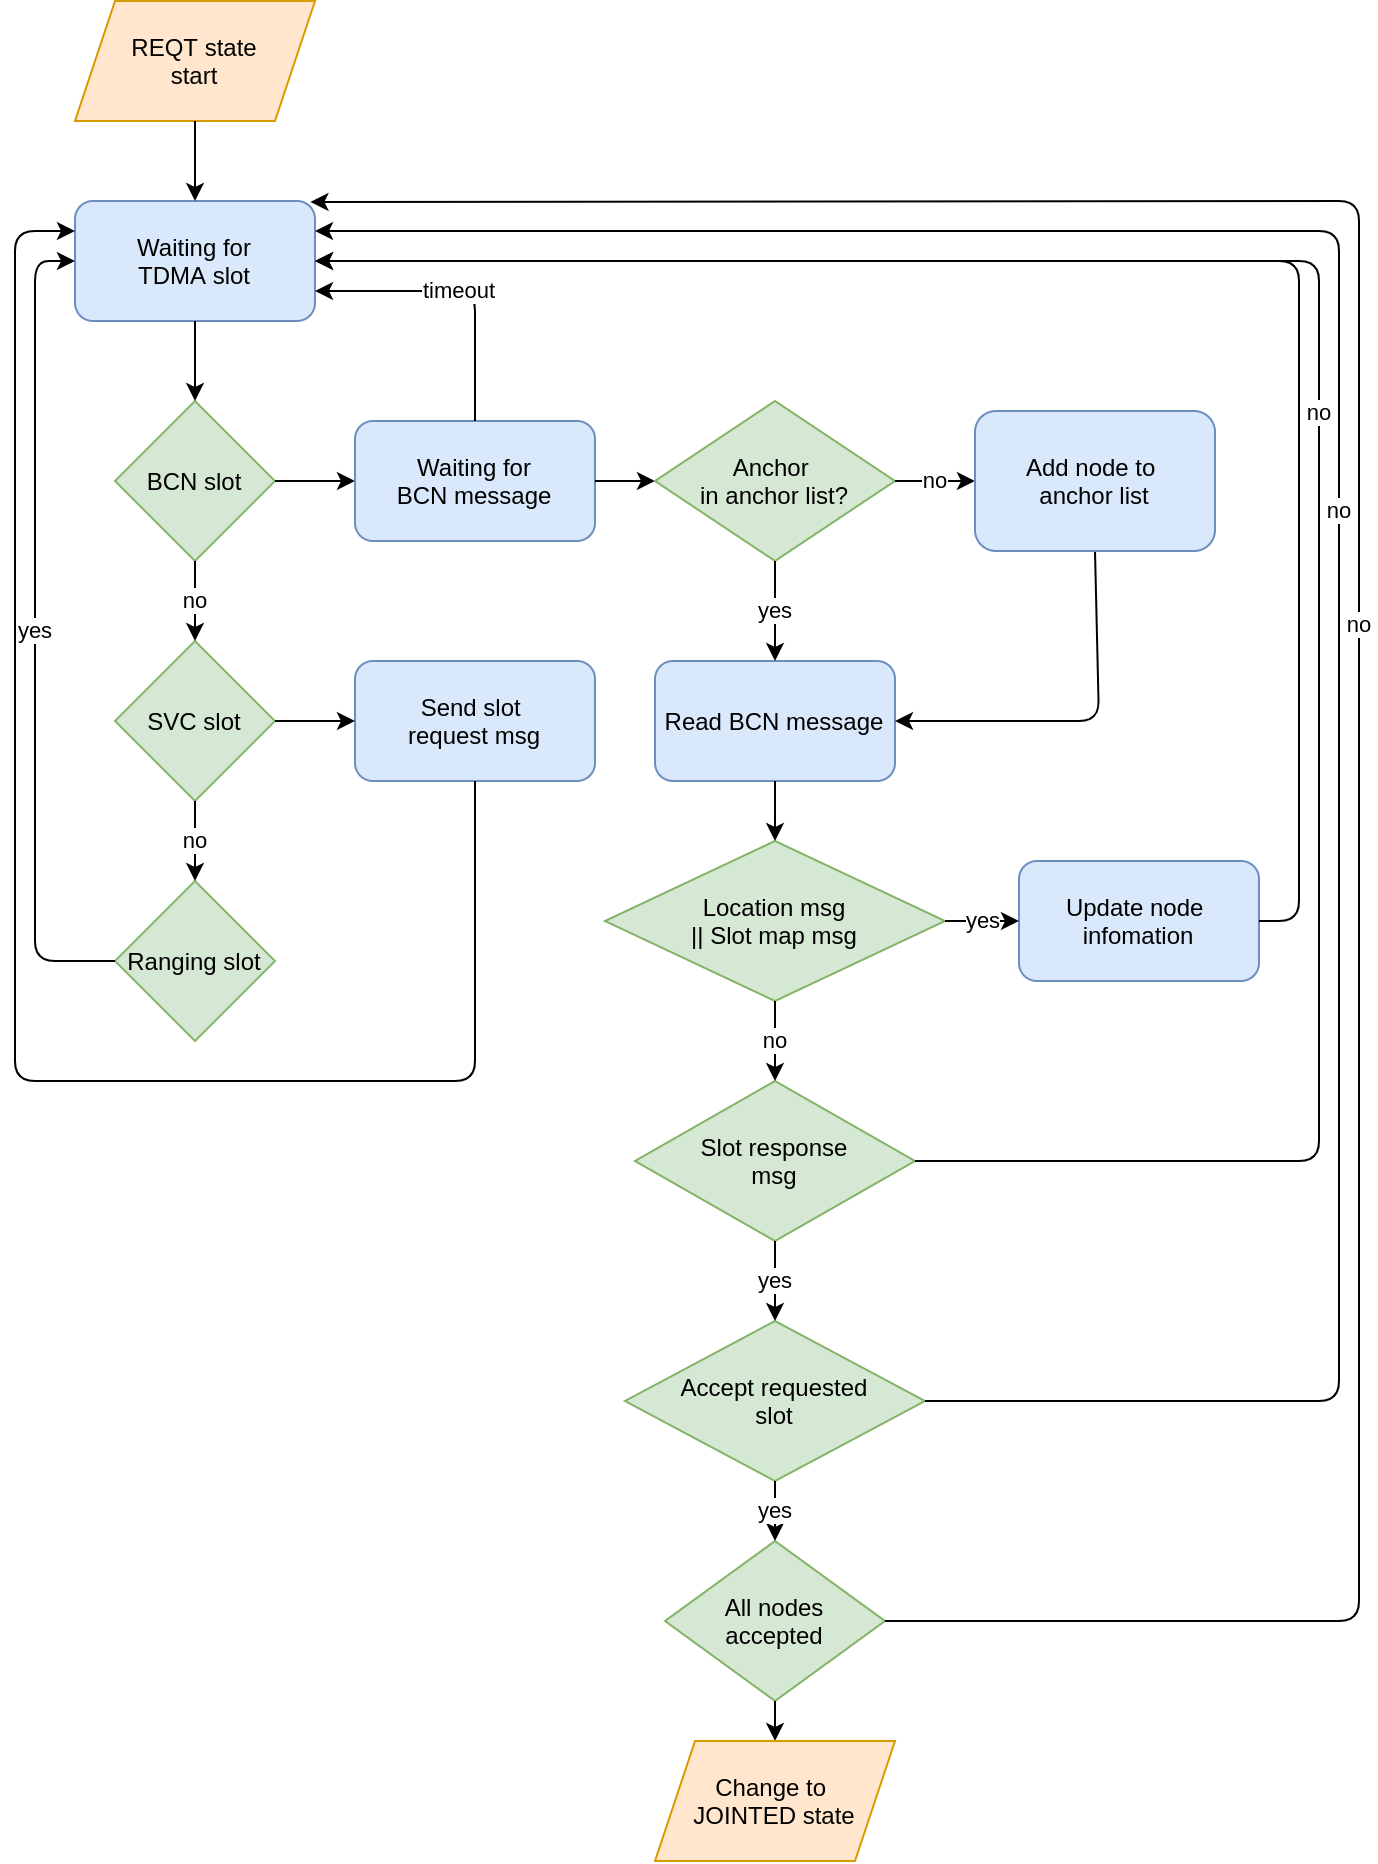
\includegraphics[scale=0.3]{REQT_flow_chart.png}
    \end{center}
    \caption{REQT state flowchart}
    \label{fig:REQT_state_flowchart}
\end{figure}

\begin{figure}[H]
    \begin{center}
        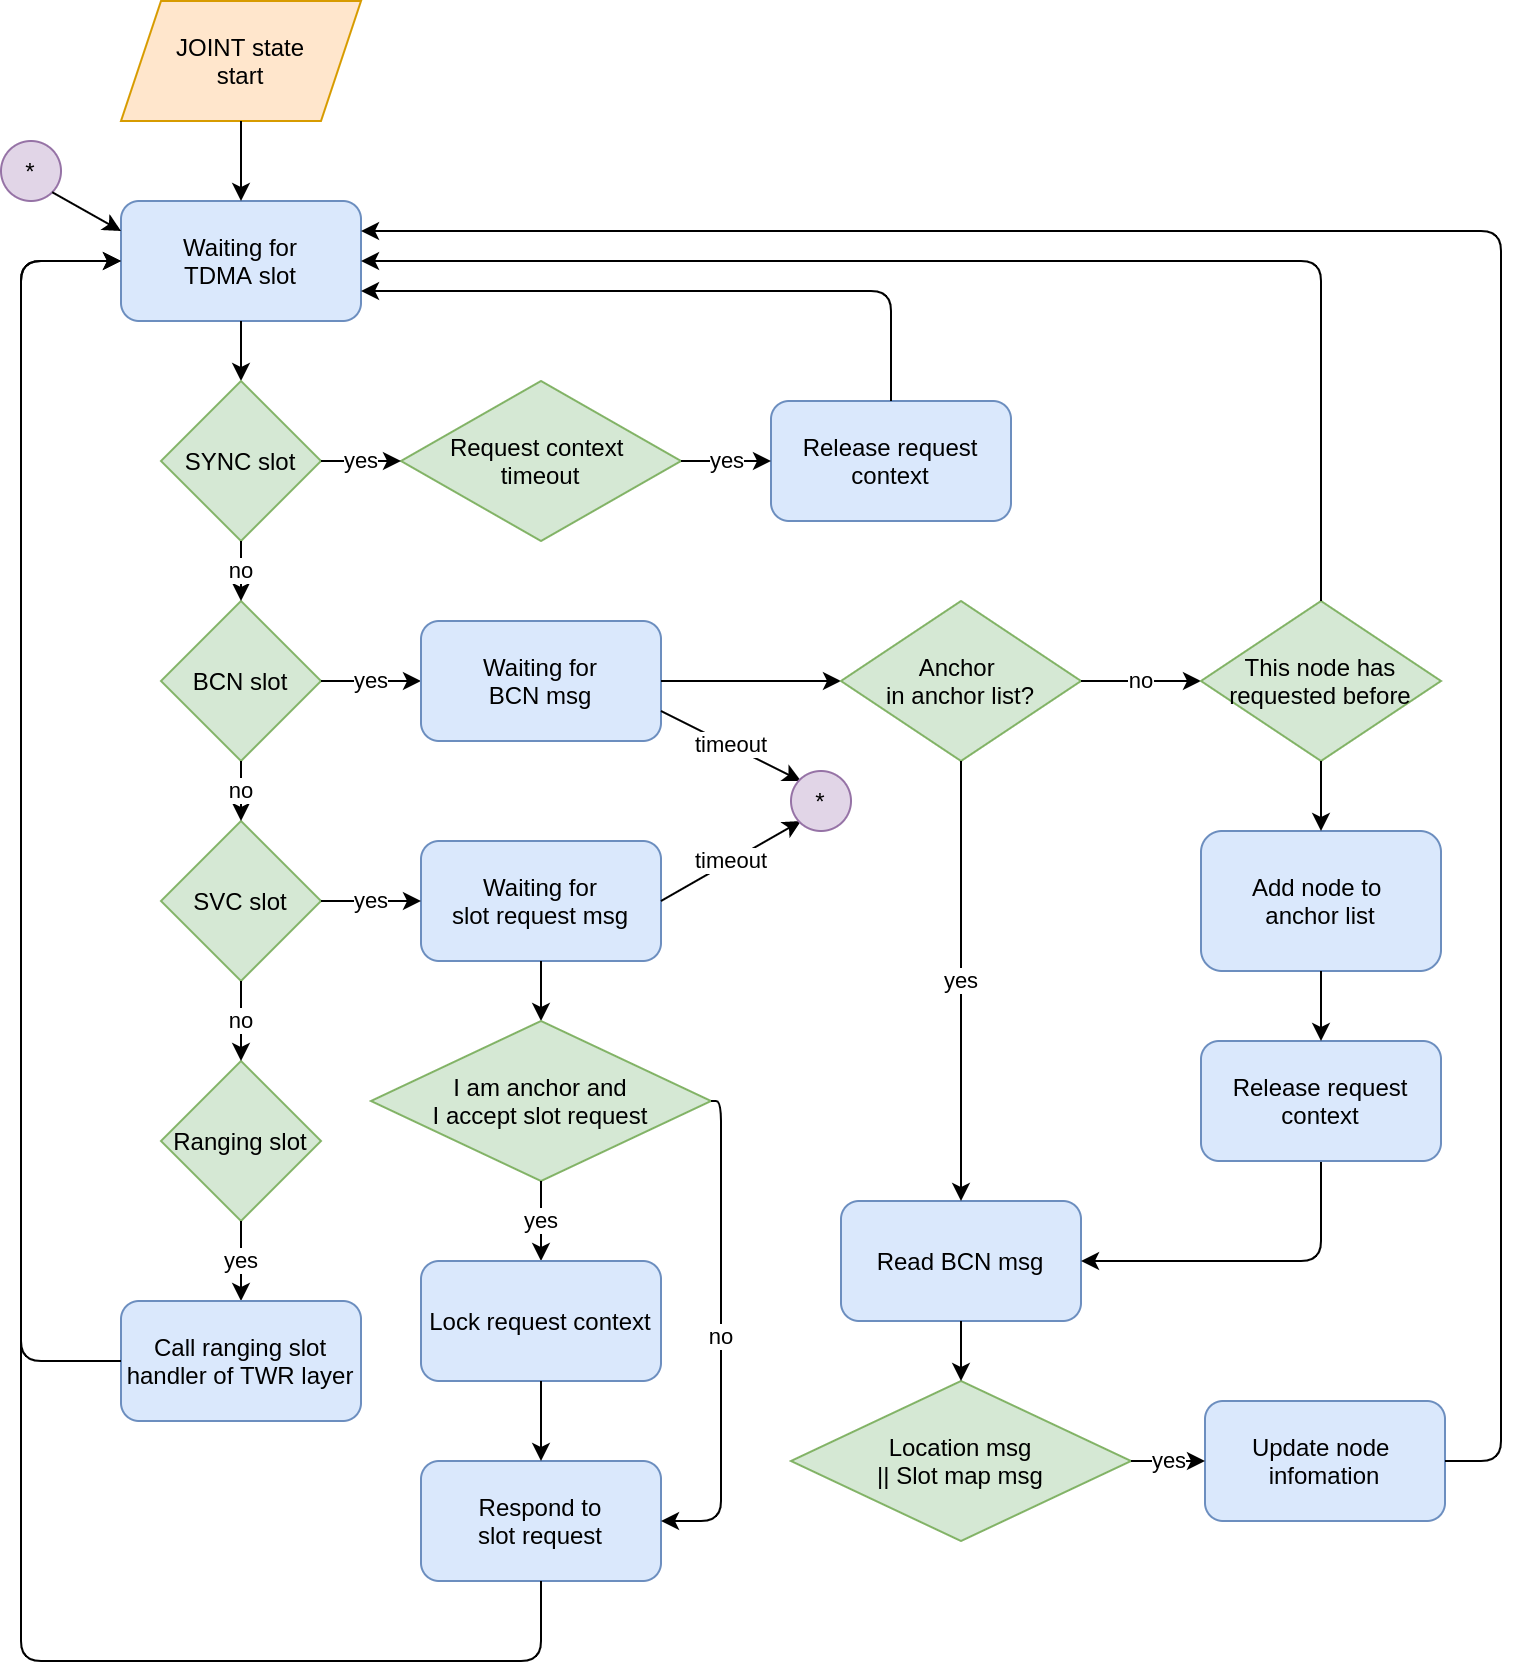
\includegraphics[scale=0.32]{JOINTED_state_flow_chart.png}
    \end{center}
    \caption{JOINTED state flowchart}
    \label{fig:JOINTED_state_flowchart}
\end{figure}

\section{Two way ranging (TWR)}
By using TWR, the need of synchronized clocks is eliminated since both the round-trip time(s) and the reply time(s) can be calculated separately using timestamps derived from each device. TWR service runs on Ranging slots of TDMA service. Figure \ref{fig:single_sided_two_way_ranging} illustrates a node sending a range request message to another node and receiving a range response message to calculate the distance.

\begin{figure}[H]
    \begin{center}
        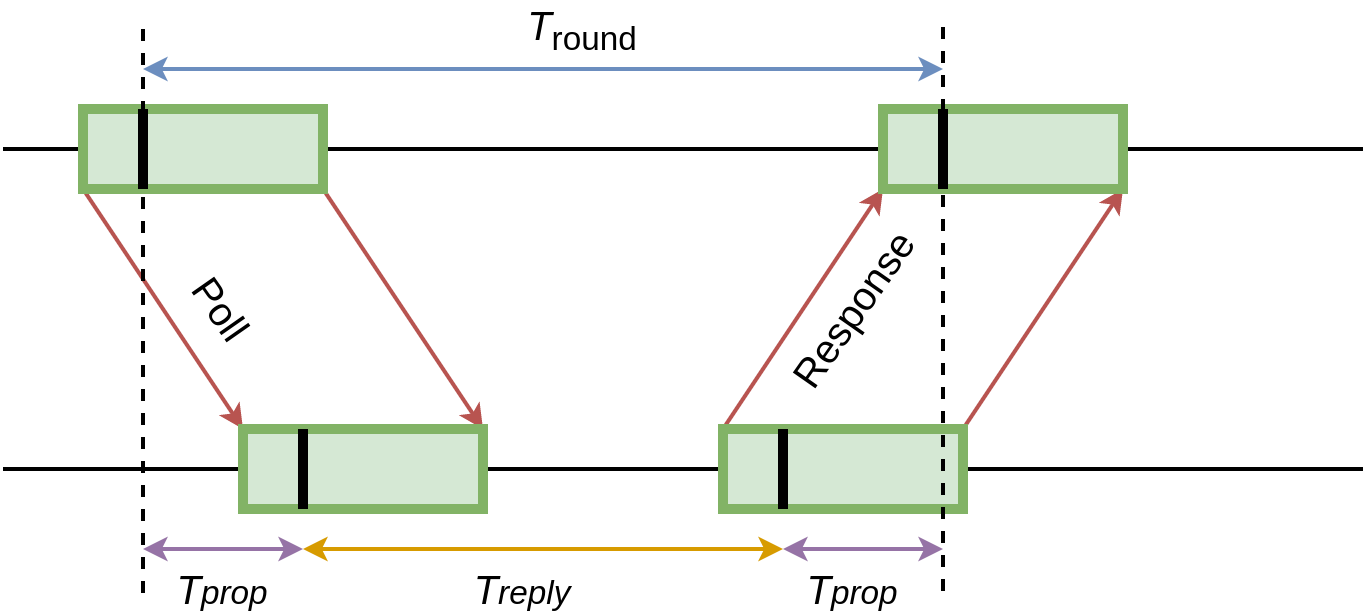
\includegraphics[width=0.8\textwidth]{single_sided_two_way_ranging.png}
    \end{center}
    \caption{Single-sided two-way ranging}
    \label{fig:single_sided_two_way_ranging}
\end{figure}

\subsection{TWR role}
\begin{itemize}
    \item TWR initiator: The tag node who sends range-request message.
    \item TWR responder: The anchor node who waits for range-request message and responses with range-response message.
\end{itemize}
\subsection{TWR frame format}
\begin{figure}[H]
    \centering
    \begin{bytefield}[bitwidth=1.1em]{32}
        \bitheader{0-31} \\
        \begin{rightwordgroup}{IEEE \\ frame \\ header}
            \bitbox{16}{frame control} & 
            \bitbox{8}{sequence number} \\ 
            \bitbox{16}{pand id} \\
            \bitbox{16}{dst address} &
            \bitbox{16}{src address}
        \end{rightwordgroup} \\
        \bitbox{16}{code} \\
        \wordbox{1}{payload}
    \end{bytefield}
    \caption{TWR frame}
    \label{fig:twr_frame}
\end{figure}

\subsubsection{Frame Control}
The Frame Control field for the standard Data frame are specified in figure \ref{fig:function_control_for_standard_data_frame}.
\begin{figure}[H]
    \centering
    \begin{bytefield}[bitwidth=2.7em, bitheight=6em]{16}
        \bitheader{0-15} \\
        \bitbox{3}{Frame Type} &
        \bitbox{3}{} &
        \bitbox{1}{PAN ID Compression} &
        \bitbox{3}{} &
        \bitbox{2}{Destination Addressing Mode} &
        \bitbox{2}{} &
        \bitbox{2}{Source Addressing Mode}
    \end{bytefield}
    \caption{Function Control for stand Data Frame}
    \label{fig:function_control_for_standard_data_frame}
\end{figure}
The Frame Type field shall be set as $b_2 b_1 b_0 = 001$ for data frame.

The PAN ID Compression field is used to indicate the presence of the PAN ID field. As both destination and source addressing information is present, the MAC sub-layer shall compare the destination and source PAN identifiers and see the PAN IDs are identical, the PAN ID Compression field is set to 1 and the Source PAN ID field is omitted from the transmitted frame. 

The Destination Addressing Mode field shall be set to  $b_1 b_0 = 10$ as the destination address field contains a short address (16 bit).

The Source Addressing Mode field shall be set to  $b_1 b_0 = 10$ as the source address field contains a short address (16 bit).

The final value for the frame control field is: \textbf{0x8841}
\subsubsection{Sequence Number}
The Sequence Number field specifies the sequence identifier for the frame

\subsubsection{Pan ID}
The Destination PAN ID field is an unsigned integer that specifies the unique PAN ID of the intended recipient of the frame. 

\subsubsection{Dst Address}
The Destination Address field with a length specified in the Destination Addressing Mode field of the Frame Control field specifies the address of the intended recipient of the frame.

\subsubsection{Src Address}
The Source Address field specifies the address of the originator of the frame. As the Source Addressing Mode field is nonzero, this field is included in the MAC frame.

\subsubsection{Code}
Code is a self-defined state variable for a TWR process. For single-sided TWR, the Code field shall be set to one of the values listed in table \ref{tab:TWR_code}.

\begin{table}[H]
\centering
\begin{tabular}{ |p{7.5cm}|c|p{7.5cm}| } 
    \hline
    UWB\_DATA\_CODE\_TWR\_INVALID & 0x0100 & Invalid TWR CODE \\\hline
    UWB\_DATA\_CODE\_SS\_TWR & 0x0110 & Single sided TWR \\\hline
    UWB\_DATA\_CODE\_SS\_TWR\_T1 & 0x0111 & Response for single sided TWR \\\hline
    UWB\_DATA\_CODE\_SS\_TWR\_FINAL & 0x0112 & Final response of single  sided TWR \\\hline
    UWB\_DATA\_CODE\_SS\_TWR\_END & 0x0113 & End of single sided TWR \\\hline
\end{tabular}
\caption{TWR code}
\label{tab:TWR_code}
\end{table}

\subsubsection{Payload}
The Frame Payload field contains information specific to individual frame types.

For the range-request frame type, the payload shall be formatted as illustrated in figure \ref{fig:twr_slot_payload}.
\begin{figure}[H]
    \centering
    \begin{bytefield}[bitwidth=1.3em]{32}
        \bitheader{0-31} \\
        \bitbox{2}{ptype} &
        \bitbox{14}{start slot id} &
        \bitbox{16}{end slot id} &
    \end{bytefield}
    \caption{TWR slot payload}
    \label{fig:twr_slot_payload}
\end{figure}

For the range-response frame type, the payload shall be formatted as illustrated in figure \ref{fig:twr_response_payload}.
\begin{figure}[H]
    \centering
    \begin{bytefield}[bitwidth=1em]{32}
        \bitheader{0-31} \\
        \bitbox{16}{reception timestamp} &
        \bitbox{16}{transmissiontimestamp} &
    \end{bytefield}
    \caption{TWR response payload}
    \label{fig:twr_response_payload}
\end{figure}

\subsection{TWR flowchart}
Flowcharts for TWR initiator and responder is shown is figure \ref{fig:twr_initiator} and \ref{fig:twr_responder}.
The initiator sends a range-request message in its slot and waits for range-response messages from responders. If a response is successfully received, it will calculate the time of light using. In the other hand, responders wait for a range-request message and respond after a fixed interval.

\begin{figure}[H]
    \centering
    \begin{subfigure}[b]{0.47\textwidth}
        \begin{center}
            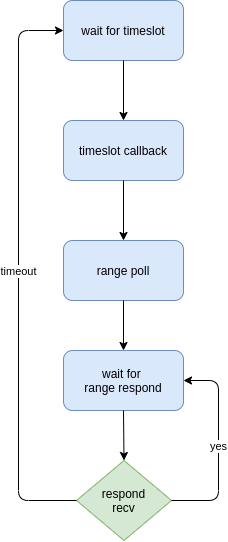
\includegraphics[scale=0.3]{twr_initiator.png}
        \end{center}
        \caption{TWR initiator flow chart}
        \label{fig:twr_initiator}
    \end{subfigure}
    \hfill
    \begin{subfigure}[b]{0.47\textwidth}
        \begin{center}
            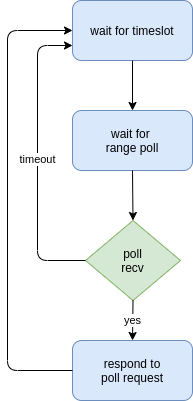
\includegraphics[scale=0.3]{twr_responder.png}
        \end{center}
        \caption{TWR responder flow chart}
        \label{fig:twr_responder}
    \end{subfigure}
    \caption{TWR flowchart}
\end{figure}

\subsection{TWR implementation}
Timestamping for each event in TWR process is precisely done by the radio IC. The host, on the other hand, calculate TOF by using equation \ref{eqn:twr_tof} as proved in figure \ref{fig:twr_timing}.
\begin{equation}
    tof = \frac{1}{2} ((t_{resp} - t_{reqt}) - (t_{trans} - t_{recp}))
    \label{eqn:twr_tof}
\end{equation}
\begin{figure}[H]
    \begin{center}
        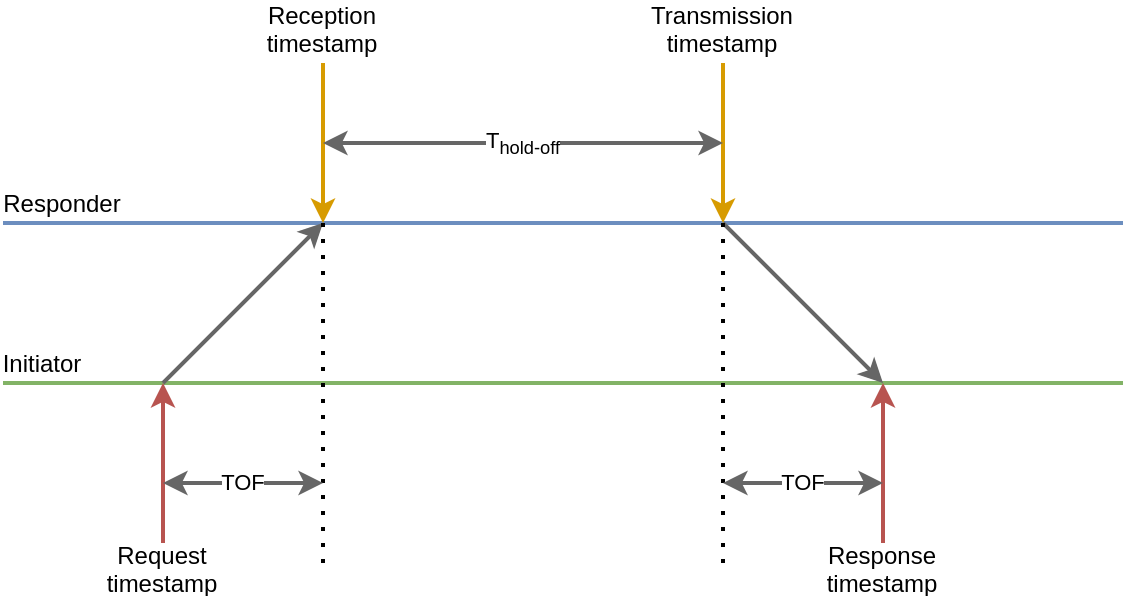
\includegraphics[width=0.8\textwidth]{twr_timing.png}
    \end{center}
    \caption{Two way ranging timing}
    \label{fig:twr_timing}
\end{figure}

\begin{figure}[H]
    \begin{center}
        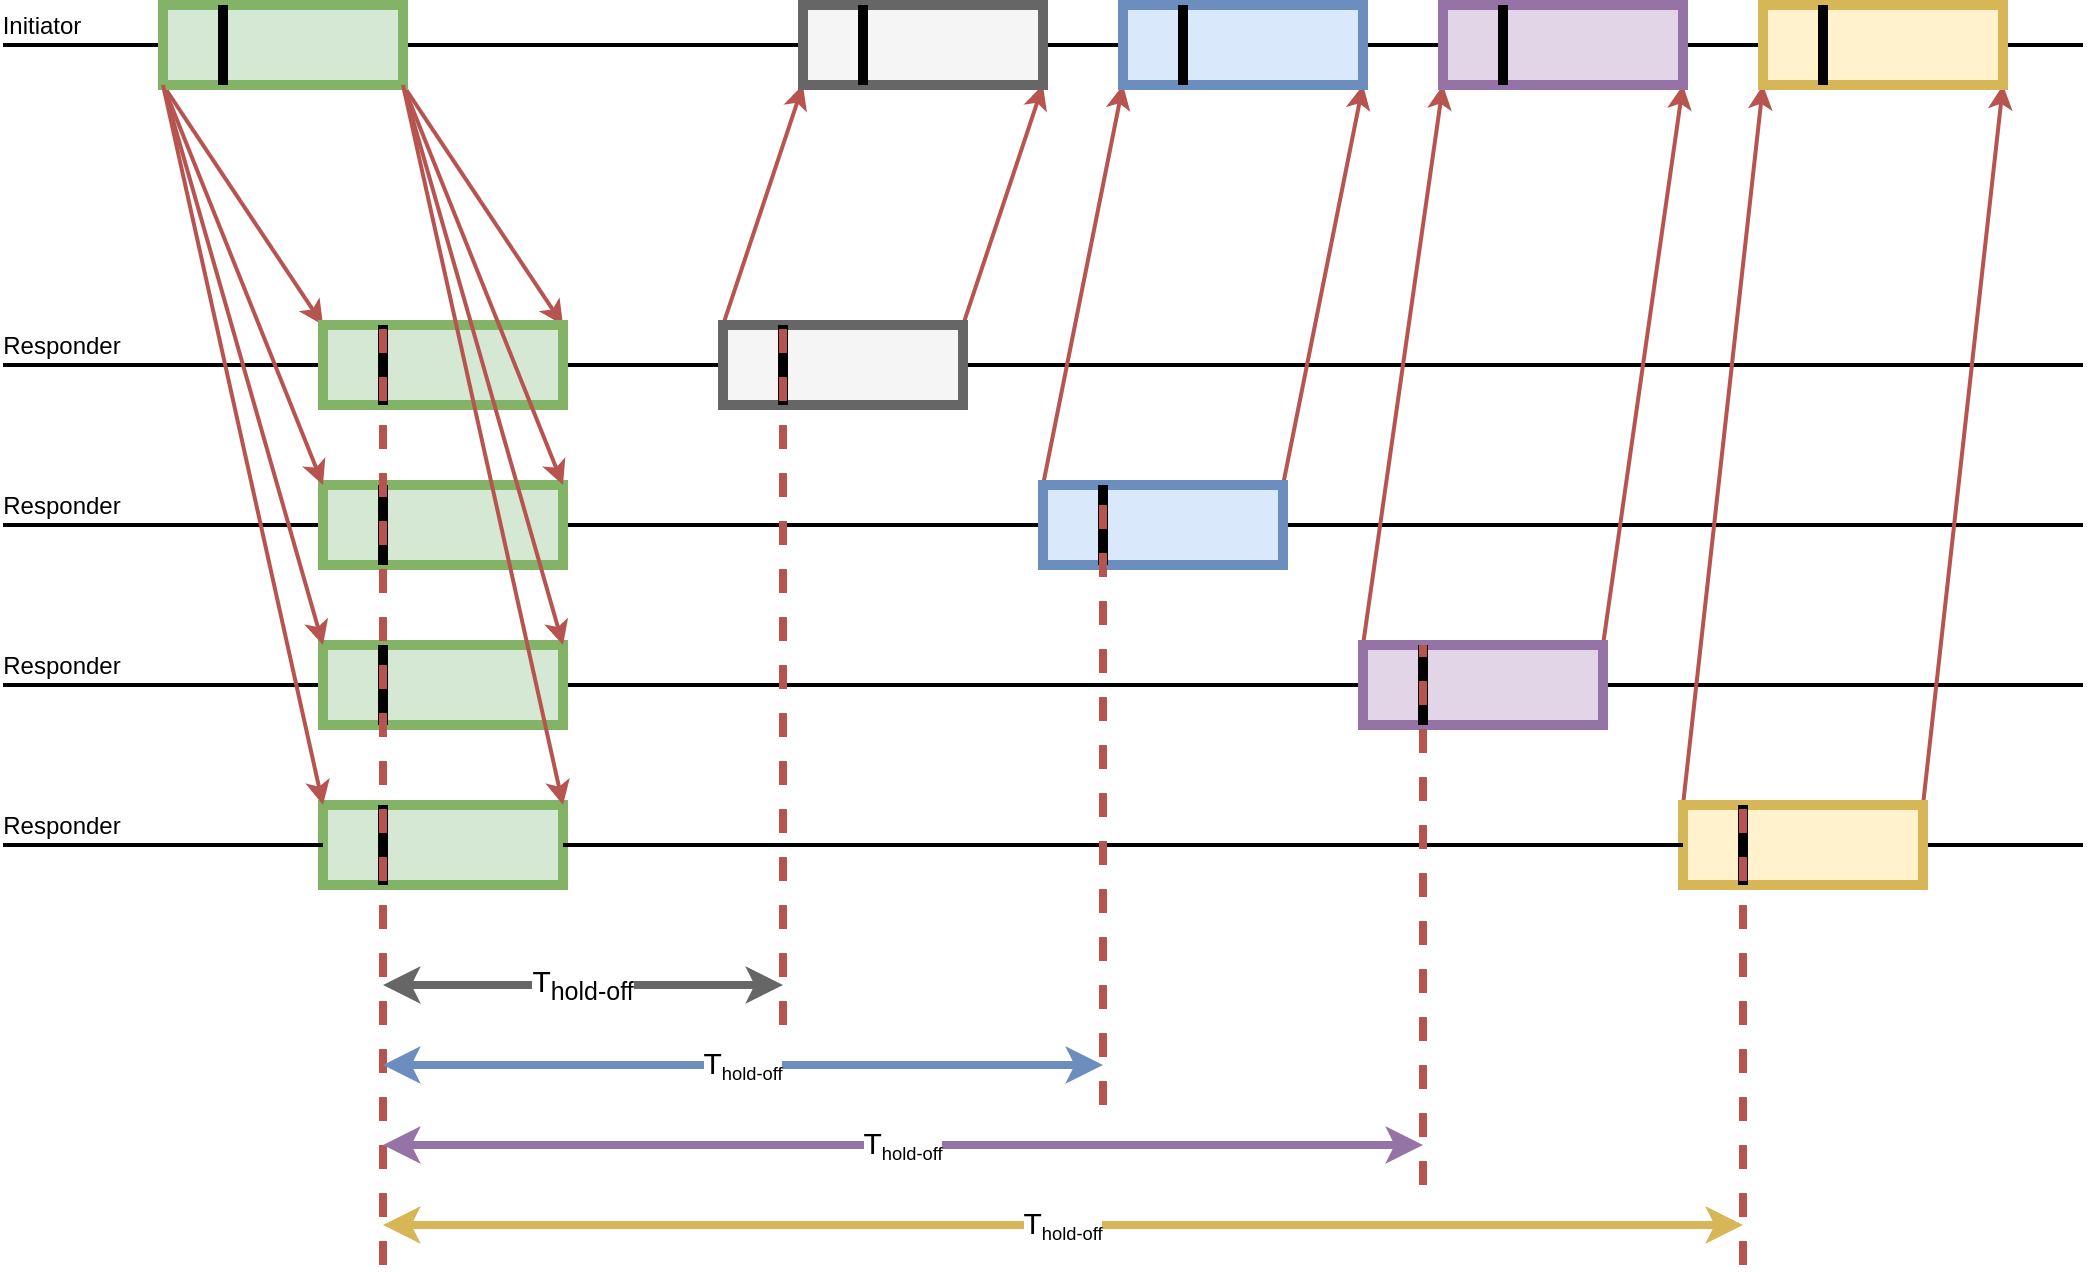
\includegraphics[width=0.8\textwidth]{single_sided_two_way_nranging.png}
    \end{center}
    \caption{Single-sided two-way n ranging}
    \label{fig:single_sided_two_way_nranging}
\end{figure}
Figure \ref{fig:single_sided_two_way_nranging} illustrates a initiator sending range request and receiving response message from 4 responder as a expected situation in the actual network.

$T_{hold-off-conf}$ is a configured value for holding the range-request message before send the range-response message.
As many anchors will response for a range-request, all anchors should respond at different time to not corrupt each other. To archive this, time slot index of anchor ($i_{slot}$) is used together with the duration of range-response frame ($T_{response-frame}$). The final hold-off time ($T_{hold-off}$) is produced using equation \ref{eqn:tdma_hold_off}.
\begin{equation}
   T_{hold-off} = T_{hold-off-conf} + i_{slot}(T_{guard} + T_{response-frame})
   \label{eqn:tdma_hold_off}
\end{equation}
Where $T_{guard}$ is used for the purpose of making response more distinct from each other.

% \begin{figure}[H]
%     \begin{center}
%         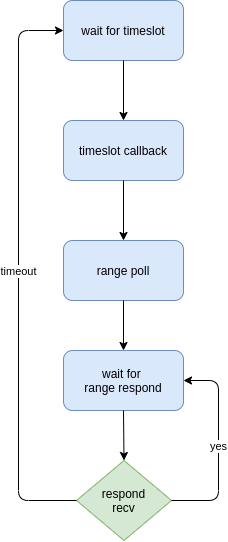
\includegraphics[scale=0.5]{twr_initiator.png}
%     \end{center}
%     \caption{TWR initiator flow chart}
%     \label{fig:twr_initiator}
% \end{figure}

% \begin{figure}[H]
%     \begin{center}
%         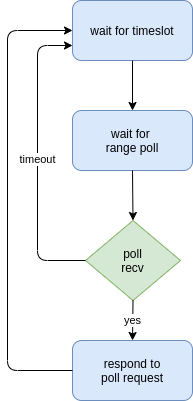
\includegraphics[scale=0.5]{twr_responder.png}
%     \end{center}
%     \caption{TWR responder flow chart}
%     \label{fig:twr_responder}
% \end{figure}

\section{Wireshark extcap for packets capturing}
While developing the whole system, Wireshark is an important tool to analyze network traffic and troubleshoot issues on the network. Wireshark has been pre-implemented for parsing 802.15.4 packet. Nevertheless, it can only capture packets from standard interfaces. The extcap interface, however, is a versatile plugin interface that allows external binaries to act as capture interfaces directly in Wireshark.

Without extcap, a capture can always be achieved by directly writing to a capture file, but the extcap interface allows for such a connection to be easily established and configured using the Wireshark GUI. The extcap subsystem is made of multiple extcap binaries that are automatically called by the GUI in a row. Extcaps may be any binary or script within the extcap directory.

How extcap make interfaces available to Wireshark? Figure \ref{fig:extcap_802_15_4} shows the principle. Wireshark creates a FIFO and pass it to the extcap program as an argument. The extcap program, on the other hand, send the received frame to the FIFO with the protocol defined by Wireshark. How the extcap program gets the frame is not important to the Wireshark. In this case, the radio module acts as a sniffer and gives its received frame to the extcap over an UART connection.

Figure \ref{fig:extcap_802_15_4} shows the interface created by a extcap program for capturing 802.15.4 frame of a UWB system.

Figure \ref{fig:wireshark_802_15_5_packet} is an example of a 802.15.4 frame analyzed by Wireshark.

\begin{figure}[H]
    \begin{center}
        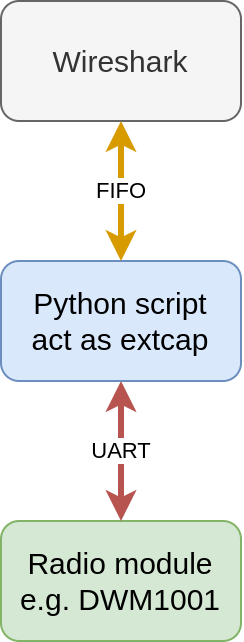
\includegraphics[width=0.15\textwidth]{extcap_802_15_4.png}
    \end{center}
    \caption{Wireshark for debugging the network}
    \label{fig:extcap_802_15_4}
\end{figure}

\begin{figure}[H]
    \begin{center}
        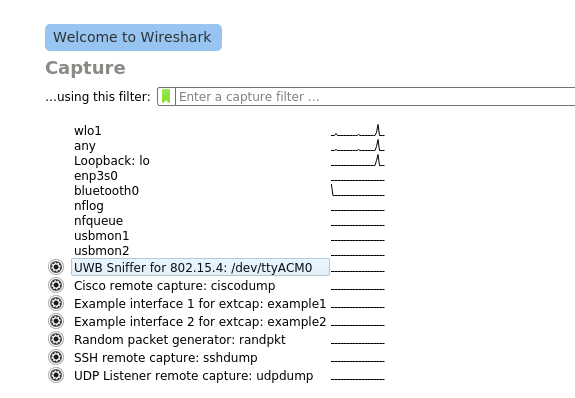
\includegraphics[width=0.7\textwidth]{wireshark_interface.png}
    \end{center}
    \caption{UWB Wireshark interface}
    \label{fig:wireshark_interface}
\end{figure}

\begin{figure}[H]
    \begin{center}
        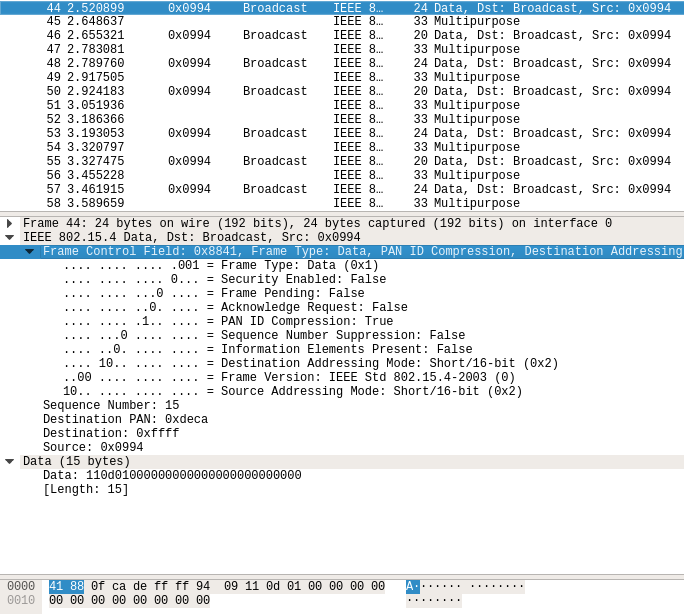
\includegraphics[width=0.7\textwidth]{wireshark_802_15_5_packet.png}
    \end{center}
    \caption{UWB 802.15.4 packet parsing}
    \label{fig:wireshark_802_15_5_packet}
\end{figure}

\bib
\end{document}